% Mechanistic Views: A Five-Axis Ontology for Mechanistic Interpretability
\pdfoutput=1

\documentclass{article}

\usepackage[preprint]{tmlr}

\def\month{06}
\def\year{2026}

\usepackage{amsmath,amssymb}
\usepackage{booktabs}
\usepackage{array}
\usepackage{enumitem}
\usepackage{graphicx}
\graphicspath{{figures/}}
\usepackage{xcolor}
\usepackage{hyperref}
\usepackage{multirow}
\usepackage{float}

% --- Macros ---
\newcommand{\Gr}{\mathrm{Gr}}
\newcommand{\R}{\mathbb{R}}
\newcommand{\calM}{\mathcal{M}}
\newcommand{\calE}{\mathcal{E}}
\newcommand{\IIA}{\mathrm{IIA}}

\title{Mechanistic Views: A Five-Axis Ontology for Mechanistic Interpretability}

\author{
Elliot Tower \\
\texttt{elliot@elliottower.ai}
}

\begin{document}
\maketitle

\begin{abstract}
Mechanistic interpretability has produced circuits, features, causal
subspaces, and activation-steered algorithms---each resting on an
implicit answer to a prior question: what kind of thing is a mechanism?
These are not terminological variants.  They differ in ontology, and
ontological differences propagate: what a mechanism \emph{is} determines
when two descriptions pick out the \emph{same} one, what \emph{evidence}
can warrant a claim, and what \emph{inferences} that claim licenses.
This paper introduces \emph{mechanistic views}: the explicit background
assumptions behind any mechanistic claim.  Each view answers five
questions: what kind of entity counts as a mechanism (ontology), when
two descriptions refer to the same one (identity), what measurements
can warrant the claim (evidence), what mathematical language expresses
it (formalism), and what phenomenon is being explained (target).
The five axes form a dependency chain: ontology constrains identity,
which constrains formalism.  We argue that many apparent disagreements
in the field arise from unstated mismatches between these axes.

A motivating walkthrough shows how a single claim---``head~9.9
is an S-inhibition head''---splits into seven distinct claims under
different views, grounded in recent empirical data on circuit overlap,
head stability, and prompt specificity.
We present an atlas of nine views, classify common methods by their
implicit view commitments, and apply the framework to four worked
examples.  Surveying 17 open problems from seven sources, we find that
8 dissolve once the view is specified, 2 become answerable once the
required evidence type is identified, and 7 arise structurally from the
limits of the view currently used to study them.
The last category is the most important: these are not puzzles waiting
for better methods but ceilings that the field's default operating
point---object ontology with activation-patching evidence---cannot
transcend.
\end{abstract}


%% ---------------------------------------------------------------
\section{Introduction}
%% ---------------------------------------------------------------

Mechanistic interpretability aims to explain what trained neural
networks are computing.  The field has made this aim concrete:
transformer circuits provide a component-level vocabulary for attention
heads and MLPs \citep{elhage2021}; induction heads account for a
mechanism involved in in-context learning \citep{olsson2022}; the
indirect object identification (IOI) circuit names the attention heads
involved in a specific syntactic task \citep{wang2022}; sparse
autoencoders recover interpretable directions from activation spaces
\citep{bricken2023,templeton2024}; causal abstraction methods test
whether high-level variables are realized in distributed representations
\citep{geiger2021,geiger2024}; and weight-space analyses recover
inter-layer communication channels and circuit structure from weight
matrices alone \citep{merullo2024,elhage2021}.

Yet the word \emph{mechanism} does not mean the same thing in all of
these cases.  In one paper a mechanism is a set of attention heads;
in another it is a functional role such as ``name mover''; in another
it is a causal subspace recovered by distributed alignment search; in
another it is a training-time transition.  These are not merely
terminological differences.  They carry different answers to five basic
questions:
\begin{enumerate}[leftmargin=*,label=(\arabic*)]
\item \textbf{Ontology}: what kind of entity counts as a mechanism?
\item \textbf{Identity}: when do two descriptions refer to the same mechanism?
\item \textbf{Evidence}: what measurements can warrant a claim about a mechanism?
\item \textbf{Formalism}: what mathematical language expresses the claim?
\item \textbf{Target}: what phenomenon is the mechanism supposed to explain?
\end{enumerate}
These questions are not new.  The philosophy of science has studied
mechanisms for decades: the Machamer-Darden-Craver (MDC) account defines
mechanisms as entities and activities organized to produce a phenomenon
\citep{machamer2000}; Glennan argues that mechanisms ground causal claims
\citep{glennan1996}; Craver develops mutual manipulability as the
criterion for constitutive relevance \citep{craver2007}; Bechtel and
Richardson study decomposition and localization as discovery strategies
\citep{bechtel1993}; and Illari and Williamson survey the diversity of
mechanism concepts across the sciences \citep{illari2012}.  What
interpretability adds is precision about the objects: neural network
mechanisms are computationally specified, fully inspectable, and amenable
to exact intervention.  What interpretability lacks is the conceptual
infrastructure that the philosophy of mechanisms provides.
\citet{williams2025} independently argue that MI needs philosophical
foundations for clarifying concepts, refining methods, and navigating
epistemic complexity.  This paper draws on that tradition to organize
the implicit commitments behind interpretability claims.

Most published work answers these questions implicitly.  The answers are
recoverable from the methods used and the conclusions drawn, but they are
not stated---and because they are not stated, disagreements that are
fundamentally ontological are argued as disagreements about experimental
design.

\paragraph{Three motivating cases.}

\textbf{The object-to-role slide.}
\citet{wang2022} establish that head~9.9 is causally necessary for
indirect object identification via activation patching.  The paper then
labels it ``an S-inhibition head''---a functional role.  These are
different claims under different views.  The ablation supports the
object claim: \emph{this component matters}.  The role label requires
independent operationalization: does S-inhibition predict behavior on
novel syntactic constructions?  No such test is reported.  This
pattern---establishing object identity by patching, then sliding into a
role label without independent evidence---is the most prevalent
methodological error in interpretability.
We call it the \textbf{object-to-role slide}, and it recurs throughout
the atlas (\S\ref{sec:atlas}), the diagnostic checklist
(Appendix~\ref{app:checklist}), and the worked examples
(\S\ref{sec:examples}).

\textbf{Cross-model comparison.}
\citet{merullo2024} report that the IOI circuit and the Colored Objects
circuit in GPT-2 Small share 78\% of their attention heads.  Under the
object view, this is a striking coincidence that invites mechanistic
comparison.  Under the role view, it is either confirmation that the
same functional roles appear across tasks, or evidence that what was
identified as ``the IOI circuit'' was actually a task-general
computational substrate misidentified as task-specific.  The two
readings have opposite implications for how transferable the IOI
findings are---and the choice between them is a view-level commitment,
not an empirical question that more patching can resolve.

\textbf{Safety-relevant inference.}
\citet{turner2024} show that adding a ``refusal direction'' to
activations suppresses refusal behavior.  The inference from ``this
steering vector suppresses refusal'' to ``this is the refusal
mechanism'' is a slide from instrumental evidence (the vector works as
a behavioral lever) to a structural conclusion (the vector identifies
the mechanism).  Under the instrumental view, the finding is complete:
the direction predicts and controls behavior.  Under the object view,
the direction must be shown to correspond to necessary components.
Under the subspace view, the direction must be stable across
distributions.  Safety monitoring that relies on steering-vector
evidence for mechanistic conclusions---without specifying which view
is operative---has an undiagnosed coherence violation at its
foundation.

\paragraph{Contributions.}
This paper makes five contributions:
\begin{enumerate}[leftmargin=*]
\item A motivating walkthrough (\S\ref{sec:motivation}) showing how one
      claim---``head~9.9 is an S-inhibition head''---reads as seven
      distinct claims under seven views, grounded in recent empirical
      data on circuit overlap \citep{merullo2024}, head stability
      \citep{bali2026}, prompt specificity \citep{franco2026}, and
      cross-model congruence \citep{sun2026}.
\item A definition of a \emph{mechanistic view} as five interlocking
      commitments---ontology, identity, evidence, formalism, and
      target---with coherence conditions linking them
      (\S\ref{sec:views}).
\item An atlas of nine views for mechanistic interpretability,
      with full axis assignments, evidence standards, discriminating
      experiments, and failure modes (\S\ref{sec:atlas}).
\item The determination chain---ontology implies identity implies
      formalism---with a five-axis methods mapping showing how common
      tools carry implicit view commitments
      (\S\ref{sec:chain}, \S\ref{sec:methods}).
\item A survey of 17 open problems from seven sources, decomposed by
      view: 8 dissolve once the view is specified, 2 become answerable
      once the required evidence type is identified, and 7 arise
      structurally from the limits of the view currently used to study
      them (Appendix~\ref{app:openprobs}).
\end{enumerate}
These are applied through four worked examples (\S\ref{sec:examples}),
six recurring decision points (\S\ref{sec:decisions}), and
cross-view promotion conditions (\S\ref{sec:promotion}).

\paragraph{Relationship to Marr's levels.}
The most well-known framework for levels of analysis in computational
science is Marr's tri-level account \citep{marr1982}: a computational
level (what is computed and why), an algorithmic level (what
representation and process), and an implementational level (how the
algorithm is physically realized).  Marr's levels organize
\emph{explanatory targets}---they ask what a system does, how it does
it, and what substrate realizes the process.  The five axes here
organize \emph{ontological commitments}---they ask what kind of object
the mechanism is, when two are the same, and what evidence can support
the claim.  Marr's levels do not distinguish views: two researchers
at the same Marr level can hold different mechanistic views (object vs.\
subspace vs.\ structural).  The nine views are complementary to Marr's
hierarchy, not a refinement of it: both are needed, and neither
subsumes the other.


%% ---------------------------------------------------------------
\section{From Claim to View: One Head, Nine Readings}\label{sec:motivation}
%% ---------------------------------------------------------------

Before defining views formally, we demonstrate why they matter by
taking a single, well-known mechanistic claim and reading it under
each view.  The claim is:

\begin{quote}
\emph{Head~9.9 in GPT-2 Small is an S-inhibition head in the
indirect object identification circuit.}
\end{quote}

This sentence appears unremarkable.  It names a component (head~9.9),
assigns it a role (S-inhibition), and places it in a context (the IOI
circuit).  Yet it carries at least six distinct commitments, and recent
empirical work shows that they come apart.

\paragraph{Object view.}
Under the object view, the claim is about a specific computational unit:
attention head~9.9 in a specific model.  The evidence is activation
patching: ablating head~9.9 degrades IOI performance.  The claim is
precise within GPT-2 Small and trivially fails cross-model---head~9.9
in Pythia-160M is a different object.  Cross-task component reuse
\citep{merullo2024} shows that head~9.9 appears in circuits for at
least four other tasks, raising the question of whether its role in IOI
is its essential function or one of many.

\paragraph{Role view.}
Under the role view, the claim is about a function: S-inhibition,
the suppression of attention to the subject token so the model can
attend to the indirect object.  The component is incidental---any head
performing S-inhibition is the same mechanism.
\citet{tigges2024} found that the same algorithmic roles
(S-inhibition, name moving, duplicate-token detection) persist across
training checkpoints and model scales, even when the specific heads
occupying those roles change.  Under the role view, this is expected:
the role is the mechanism, and the component is a variable realization.
Under the object view, this is a different mechanism at each scale.

\paragraph{Subspace view.}
Under the subspace view, the relevant entity is not head~9.9 but the
subspace of the residual stream at layer~9 that encodes the
subject--object distinction.  \citet{bali2026} measured attention-head
stability across random seeds and found mid-layer head assignments
unstable (stability~$\approx$0.70), while residual-stream subspaces
remain stable as measured by centered kernel alignment.
Under the subspace view, this result makes the object-level description
unreliable and the subspace-level description robust: the computation
is stable, but which head implements it is not.

\paragraph{Structural view.}
Under the structural view, the relevant object is the gauge-invariant
information flow: the composition score $\|W_{O,\text{9.9}} W_{K,v}\|_F$
for downstream heads~$v$ that read from head~9.9.
A computation-preserving reparameterization (e.g., rotating
$W_Q$~and~$W_K$ by $R$ and $R^{-1}$) changes the individual weight
matrices but not the composition score.  If the activation-patching
result survives such reparameterizations, the claim is structural;
if it does not, it is basis-dependent.

\paragraph{Process view.}
Under the process view, the question is \emph{when} head~9.9 acquired
the S-inhibition function.  \citet{olsson2022} showed that induction
heads form via phase transitions at specific training steps, with
composition scores between heads increasing sharply at the transition.
Does S-inhibition form similarly?  The answer requires checkpoint
analysis that neither the original IOI paper nor subsequent
replications provide.  Under the process view, the mechanism is
the formation trajectory, not the final-checkpoint circuit.

\paragraph{Contrastive view.}
Under the contrastive view, the S-inhibition claim is defined relative
to a foil: head~9.9 suppresses attention to the subject
\emph{compared to what}?  \citet{franco2026} showed that even within
IOI, different prompt templates (ABBA vs.\ BABA) activate different
circuit structures.  The signals flowing through head~9.9 differ between
templates---negative cosine similarity in one, near-zero in another.
The contrastive view says these are different mechanisms, because the
foil (which template) changes what the head is contrasted with.

\paragraph{Perspectival view.}
Under the perspectival view, each of the above is a partial projection.
Activation patching reveals the object-level shadow; DAS reveals the
subspace-level shadow; weight-space composition scores reveal the
structural shadow.  \citet{sun2026} found that within model families,
interpretive equivalence is high (congruence 0.89--0.99), but across
families it collapses to~0.13.  The perspectival view interprets this
as method-relative structure: a single method identifies a mechanism
within a family, but the identification does not transport to a
different family because the measurement context has changed.

\paragraph{What this walkthrough shows.}
The sentence ``head~9.9 is an S-inhibition head'' is not one claim.
It is at least seven, depending on whether the speaker means a
specific component (object), a functional role (role), a causal
subspace (subspace), a gauge-invariant structure (structural), a
formation event (process), a foil-relative difference (contrastive),
or a method-projected observation (perspectival).  The empirical
data---Merullo's 78\% overlap, Tigges's cross-scale persistence,
Bali's head instability, Franco's prompt specificity, Sun's
within-family congruence---each supports a different reading and
undermines others.

The framework developed in the following sections provides the
vocabulary to state which reading is intended, check whether the
evidence supports it, and identify when a disagreement between
researchers is actually a mismatch between unstated views.


%% ---------------------------------------------------------------
\section{Mechanistic Views}\label{sec:views}
%% ---------------------------------------------------------------

\subsection{What a Mechanistic View Is}

A mechanistic view is a background commitment that a researcher makes,
explicitly or implicitly, when they ask what a mechanism is.  When made
explicit, a view answers five questions:

\begin{enumerate}[leftmargin=*, label=(\roman*)]
\item \textbf{Ontology}: what kind of entity counts as a mechanism?
      (Concrete components, functional roles, causal subspaces,
      gauge-invariant structures, formation processes, etc.)
\item \textbf{Identity}: when do two descriptions refer to the same
      mechanism?  (Component overlap, role equivalence, subspace
      proximity, gauge-orbit membership, etc.)
\item \textbf{Evidence}: what measurements can support what claims?
      (Activation patching, DAS/IIA, weight-space scores, checkpoint
      analysis, etc.---and critically, which claims each measurement
      type can and cannot support.)
\item \textbf{Formalism}: what mathematical language expresses the
      claim?  (Directed graphs, Grassmannian geometry, fiber bundles,
      dynamical systems, etc.)
\item \textbf{Target}: what phenomenon is the mechanism supposed to
      explain?  (A specific behavior, a functional class, a
      representational variable, a computation class, etc.)
\end{enumerate}

The identity criterion should be an equivalence relation (reflexive,
symmetric, transitive).  This is not automatic: some informal notions
of mechanism identity in the literature are not transitive.  For
example, saying mechanisms $A$ and $B$ are ``related'' by shared
components, and $B$ and $C$ are ``related'' by shared function, does
not imply $A$ and $C$ are the same mechanism.  Requiring transitivity
forces precision.

\subsection{Coherence}\label{sec:coherence}

Not all combinations of answers are coherent.  A view is coherent when
its five components fit together:

\begin{enumerate}[leftmargin=*, label=(\roman*)]
\item \textbf{Identity is grounded}: the identity criterion is
      definable in terms of the ontology and the formalism.  (A view
      whose identity criterion involves objects not in its own ontology
      is incoherent.)
\item \textbf{Evidence tracks identity}: measurements should not
      distinguish objects that the identity criterion declares
      equivalent.  (Evidence that discriminates within an identity
      class is tracking a finer-grained ontology than the one
      declared.)
\item \textbf{Formalism is expressive}: every ontological object has
      a representation in the formalism, and identity can be checked
      within it.
\end{enumerate}

When a view is incoherent---when its evidence distinguishes things its
identity criterion says are the same---the result is unresolvable
disagreement.  No additional experiment of the same type can help:
each new measurement either agrees with the identity criterion (offering
no information about the discrepancy) or disagrees (adding another
conflict).

This is not an abstract concern.  A common pattern in interpretability
is to declare that mechanisms are gauge-invariant structures (structural
view ontology) but then to use activation-patching results as evidence
of mechanism presence without checking gauge invariance.  If the
patching result changes under a reparameterization that preserves
computation, it is distinguishing objects that the structural view says
are identical---and no amount of additional activation-patching evidence
can resolve this mismatch.  The disagreement between patching advocates
and DAS advocates often has this structure: the participants hold
different implicit views, so they are literally arguing about different
kinds of objects.

\subsection{The Five Axes}\label{sec:axes}

We organize the five components into named axes.  The axes are not
independent: as coherence requires, choices on one axis constrain the
others.

\paragraph{Ontology ($O$).}
What kind of entity counts as a mechanism \citep{quine1948}?
Options include: concrete
model components (heads, neurons, MLP sublayers, SAE dictionary
elements), functional roles (descriptions of what a component does
independently of which component does it), causal subspaces (linear or
nonlinear submanifolds of the residual stream that mediate a causal
variable), gauge-invariant structures (equivalence classes of weight
configurations under symmetries that preserve the computation),
temporally extended processes (formation pathways or execution
trajectories), points in a stratified mechanism space, measurement
perspectives, and predictive models.

\paragraph{Identity ($\sim$).}
When do two mechanism descriptions denote the same mechanism?  Options
include: component overlap ($x \sim y$ iff they name the same set of
heads or neurons), role equivalence ($x \sim y$ iff they specify the
same functional input--output mapping), subspace proximity ($x \sim y$
iff the principal angles between the causal subspaces are all below a
threshold $\theta$, i.e.\ geodesic distance on $\Gr(k,d)$ is small),
gauge-orbit membership ($x \sim y$ iff there exists a computation-preserving
symmetry $g$ with $g \cdot x = y$), and dynamical-basin membership
($x \sim y$ iff the formation trajectories converge to the same
attractor).

\paragraph{Evidence ($E$).}
What measurements can support what claims?  Key distinctions: activation
patching establishes causal relevance of components under a fixed
distribution; DAS/IIA with linear alignment constraints measures causal
subspace identity; weight composition scores measure structural
information flow independent of any input distribution; checkpoint
analysis establishes formation dynamics; multi-method robustness tests
perspectival convergence.  The formal epistemology of evidence
accumulation \citep{earman1992,howson1989} suggests that independent
evidence converges faster than correlated evidence---a principle that
grounds the triangulation requirement in the perspectival view.

\paragraph{Formalism ($F$).}
What representational language is appropriate?  Directed graphs (circuits);
functional decompositions (roles); Grassmannian geometry $\Gr(k,d)$
(subspaces); fiber bundles and gauge groups (structural view); dynamical
systems and phase portraits (process view); Whitney stratifications
(stratified view); measurement algebras (perspectival view).

\paragraph{Target ($T$).}
What is the mechanism supposed to explain?  A specific behavioral output
on a specific distribution; a functional class across models; a
representational variable across inputs; a computation class across
parameterizations; a formation event; a resolution-relative phenomenon;
or a behavioral prediction.

%% ---------------------------------------------------------------
\section{An Atlas of Views}\label{sec:atlas}
%% ---------------------------------------------------------------

We identify nine views.  Six are \emph{descriptive}: they characterize
views already operative in published work (Object, Role, Subspace,
Process, Instrumental, Contrastive).  Three are \emph{programmatic}:
they articulate views that are implicit in emerging research directions
but do not yet have widely adopted methods (Structural, Stratified,
Perspectival).
Table~\ref{tab:atlas} gives the full axis assignments.
The views are not mutually exclusive: a single paper may use several,
and convergence across views constitutes stronger evidence than any
single view.  The point is to distinguish them so that each view's
commitments and limitations can be assessed independently.

\begin{table}[H]
\centering
\small
\setlength{\tabcolsep}{4pt}
\begin{tabular}{p{0.10\linewidth}p{0.15\linewidth}p{0.15\linewidth}p{0.17\linewidth}p{0.15\linewidth}p{0.15\linewidth}}
\toprule
\textbf{View} & \textbf{Ontology ($O$)} & \textbf{Identity ($\sim$)}
  & \textbf{Evidence ($E$)} & \textbf{Formalism ($F$)} & \textbf{Target ($T$)} \\
\midrule
Object
  & Concrete part: head, neuron, feature
  & Component overlap
  & Ablation, activation patching
  & Directed graph
  & Specific behavior \\[3pt]
Role
  & Functional role in computation
  & Role equivalence (same I/O mapping)
  & Role-specific causal tests, cross-model
  & Functional decomposition
  & Functional class \\[3pt]
Subspace
  & Causal subspace of residual stream
  & Same projector; $d_{\Gr} < \theta$
  & DAS/IIA (linear), subspace stability
  & $\Gr(k,d)$
  & Representational variable \\[3pt]
Structural
  & Gauge-invariant relational structure
  & Gauge-orbit membership
  & Holonomy, comp. scores, reparameterization
  & Fiber bundle quotient
  & Computation class \\[3pt]
Process
  & Formation trajectory or execution regime
  & Same trajectory type or dynamical basin
  & Training checkpoints, formation knockouts
  & Dynamical system
  & Mechanism origin \\[3pt]
Stratified
  & Point in stratified mechanism space
  & Same stratum + local equivalence
  & Dimensionality tests, localization diagnostics
  & Whitney stratification
  & Resolution-relative phenomenon \\[3pt]
Perspectival
  & Projection of mechanism onto context
  & Cross-method coherence
  & Multi-method robustness
  & Measurement algebra
  & Method-relative observation \\[3pt]
Instrumental
  & Useful predictive or interventional model
  & Predictive equivalence
  & Forecast accuracy, intervention utility
  & Model theory
  & Behavioral prediction \\[3pt]
Contrastive
  & Difference relative to a foil
  & Same contrastive pattern across foil set
  & Foil-varied patching, contrastive ablation
  & Contrastive explanation
  & Why $P$ rather than $Q$ \\
\bottomrule
\end{tabular}
\caption{The nine mechanistic views with full axis assignments.}
\label{tab:atlas}
\end{table}


\subsection{Object View}

The object view treats mechanisms as concrete model components: specific
attention heads, neurons, MLP sublayers, or sparse autoencoder dictionary
elements.  It is the implicit view in circuit diagrams.  The IOI circuit
as reported by \citet{wang2022}---26 attention heads organized into
functional groups---is an object-level description: the claim is about
those specific computational units.

\paragraph{Identity.}
Two circuit descriptions refer to the same mechanism iff they name the
same components.  This is precise within a model but trivially fails
cross-model: a head in GPT-2 Small is not an object in Pythia-160M.

\paragraph{Evidence.}
Ablation and activation patching are the natural evidence types.  Removing
a component's activation and observing behavioral degradation establishes
causal necessity; replacing it with a counterfactual activation establishes
causal sufficiency relative to that counterfactual.  The method is
strongest when the component set is stable across prompt distributions
and the ablation effect is large and specific.

\paragraph{Failure modes.}
\emph{Role inflation}: a component is identified by patching, then labeled
with a role (``name mover,'' ``induction head'') that implies richer
mechanistic content than the object-level evidence supports.  The component
identity is established; the role is a hypothesis.  \emph{Distribution
sensitivity}: the circuit identified by patching on one distribution may
differ substantially on another, meaning the claimed object-level mechanism
is distribution-relative.

\paragraph{Discriminating experiment.}
To test whether the object view is appropriate: ablate the identified
component set and test whether behavioral degradation is (a)~specific to
the behavior the mechanism is supposed to implement and (b)~stable across
prompt distributions.  If (b) fails, the object-level description is
distribution-relative and a role or subspace description may be more
appropriate.

\paragraph{Compositional variant.}
A natural refinement of the object view defines mechanisms not by
component indices but by the computation graph they implement: each edge
is a tensor operation, and two circuits are the same if their
computation graphs are isomorphic.  This is strictly more
abstract than component overlap (it ignores which head occupies each
node) but more concrete than the role view (it preserves graph
structure, not just input--output behavior).  Transcoder-based
circuit analysis implicitly adopts this variant.  We treat it as a
variant of the object view rather than a separate view because it
shares the same evidence types and failure modes; the difference is
in the identity criterion only.

\subsection{Role View}

The role view treats mechanisms as functional roles that can be realized
by different components---the role is a universal that can be multiply
instantiated \citep{lewis1972}.  ``Name mover'' is a role: it describes
what a component does (copy a name token to the output position), not
which head does it.  The role view explains why functionally equivalent
components across different models can be meaningfully compared.

\paragraph{Identity.}
Same functional input--output role, possibly in different components or
models.  Role identity requires a specification of the role that is
independent of the discovery procedure (i.e., not merely ``does what
this head does'') and tests that go beyond the ablation that revealed
the component.

\paragraph{Evidence.}
Role-specific predictions that are not entailed by mere causal relevance.
For a name-mover role claim: the weight-space signature of $W_{OV}$
should encode a copying operation; the head should perform this function
on novel prompts; a head in a different model with the same $W_{OV}$
signature should earn the same label.  The object-to-role slide is
a common source of overclaiming: establishing
that head 9.9 is causally necessary for IOI does not establish that it
is a name mover---the ablation evidence supports the object claim
(this component matters) but not the role claim (this component performs
a specific function) until the role is independently operationalized
and tested.

\paragraph{Failure modes.}
\emph{Role proliferation}: a new role label is coined for each component
discovered, re-describing the data without adding explanatory content.
\emph{Underdefined roles}: role labels are informal enough to be true of
any component, making them unfalsifiable.

\paragraph{Discriminating experiment.}
Take the role specification and apply it to a model in which the
original component has been ablated.  If the role is real, either another
component should take over (backup mechanism) or the behavior should
degrade in a specific role-consistent way.  If no such prediction is
confirmed, the role label has not been independently validated.

\subsection{Subspace View}

The subspace view treats mechanisms as low-dimensional causal subspaces
of the residual stream.  The key observation is that distributed
alignment search \citep{geiger2021,geiger2024} identifies not a component
but a rotation of the activation space: the causal variable is encoded
in a subspace that may span many components.  If alignment matrix $Q$
and its rotation $QR$ both achieve the same interchange intervention
accuracy (IIA), the relevant object is the subspace $\mathrm{span}(Q)$,
not the matrix $Q$.

\paragraph{Identity.}
Two subspace mechanisms are the same iff they project onto the same
subspace of $\mathbb{R}^d$: same projector $QQ^\top$, or equivalently
small geodesic distance on $\Gr(k,d)$.  This is basis-invariant and
can be meaningful cross-model when corresponding residual streams can
be aligned.

\paragraph{Evidence.}
The subspace view requires evidence that a specific subspace mediates a
causal variable, not merely that a search over subspaces finds one that
works.  Native subspace evidence includes: SVD or eigendecomposition of
weight matrices recovering the subspace without activation data;
Grassmannian distance between subspaces recovered by independent methods
(weight vs.\ activation); and subspace stability across prompt
distributions.  DAS and IIA are often cited as subspace evidence, but as
Table~\ref{tab:methods} shows, DAS is more precisely a Role-view method
with a borrowed subspace parameterization: it validates by intervention
success (role equivalence), not by Grassmannian distance.  DAS can
\emph{discover} a candidate subspace, but confirming that it is the
causally relevant subspace---rather than merely a subspace that permits
successful interchange---requires convergent evidence from weight-space
analysis.

\textbf{Alignment class constraints.}  \citet{sutter2025}\label{sutter}
showed that unrestricted nonlinear alignment maps achieve $100\%$ IIA
even on randomly initialized models, making DAS vacuous without
structural constraints on the alignment class.  Subspace-view claims
therefore require either linear alignment or alignment constrained to
respect the transport structure induced by the weight matrices.  Subject
to this constraint, subspace stability (eigenvalue gap between the causal
subspace and its complement) is the natural diagnostic.  This constraint
recurs throughout the atlas: it limits the evidential range of DAS
(Section~\ref{sec:methods}), appears in the diagnostic checklist
(Appendix~\ref{app:checklist}), and is the primary threat to subspace
claims in the worked examples.

\paragraph{Failure modes.}
\emph{SAE confusion}: sparse autoencoder features are dictionary elements
that minimize reconstruction loss; causal subspaces are directions that
mediate specific causal paths.  These are different objectives and can
disagree.  An SAE feature is a hypothesis about a one-dimensional
subspace mechanism, not a confirmed subspace claim.  \emph{Unconstrained alignment vacuousness} (see above):
reporting high IIA without specifying the alignment class allows any
model to be assigned any causal structure.

\paragraph{Discriminating experiment.}
Verify that the identified subspace is stable: the subspace recovered
by DAS on a held-out distribution should have small geodesic distance
from the training-distribution subspace.  Also confirm that
an aligned basis-change (within the subspace) does not change the IIA,
while a rotation that takes vectors out of the subspace does reduce it.

\subsection{Structural View}

The structural view treats mechanisms as equivalence classes of
implementations under transformations that preserve the computation.
The relevant object is not a head index, a basis vector, or a specific
projection---it is the orbit of implementations related by the symmetry
group of the transformer's weight space.  Two weight configurations
that implement the same computation via different parameterizations are
the same mechanism under this view.

The natural formalism borrows from differential geometry:
gauge orbits, transport maps, and holonomy groups
\citep{nakahara2003}.  This view is largely programmatic---the
formalism exists, but systematic empirical application to neural
networks does not yet.

\paragraph{Identity.}
Gauge-orbit membership: $x \sim y$ iff there exists a computation-preserving
symmetry $g$ (such as a scale transformation, a rotation of a head's
query-key subspace paired with an inverse rotation of its output, or a
permutation of neurons) such that $g \cdot x = y$.  Holonomy fingerprints
provide a finer criterion: the holonomy group of the transport map
induced by a mechanism's weight matrices is an invariant that does not
change under gauge transformations.

\paragraph{Evidence.}
Gauge-invariant measurements: weight-space composition scores
$\|W_{O,u} W_{K,v}\|_F$ measure information flow capacity independently
of basis choice \citep{elhage2021,merullo2024}; holonomy measurements; and
reparameterization-stability tests (check that a result survives
computation-preserving rescalings of the weights).

\paragraph{Failure modes.}
\emph{False gauge invariance}: claiming structural equivalence without
verifying that the symmetry actually preserves the computation.
\emph{Architectural prior confound}: structural features that
discriminate trained from randomly initialized models may be detecting
architecturally privileged positions rather than learned structure.

\paragraph{Discriminating experiment.}
Apply a known computation-preserving symmetry (e.g., scale by $\lambda$,
counter-scale by $\lambda^{-1}$) to the weights of a component and
retest the activation-space evidence.  If the activation-space result
changes, the original result was not gauge-invariant and is not a
structural-view claim.

\subsection{Process View}

The process view treats mechanisms as temporally extended.  A mechanism
is not merely a final-checkpoint artifact but a formation process, an
execution trajectory, or a dynamical regime---what Darden calls
``reasoning about mechanisms in the making'' \citep{darden2006}.  This
view is natural for phenomena where the how of learning is itself
mechanistically relevant:
the induction head mechanism, for instance, forms via a phase transition
at a specific training step \citep{olsson2022}---this is process-level
structure that is not recoverable from the final checkpoint alone.

\paragraph{Identity.}
Same trajectory type or dynamical basin.  Two processes are the same
mechanism if they follow the same formation pathway, occupy the same
attractor, or exhibit the same phase-transition structure.  This notion
of identity is less developed than component or subspace identity, and
formalizing it is an open problem.

\paragraph{Evidence.}
Checkpoints, gradient flow, loss-curve structure, and formation knockouts.
A mechanism claim under the process view cannot be supported by
final-checkpoint analysis alone.  The induction head formation result
provides a clear example: the phase change at a specific training step
is visible in the composition score evolution, and this is process-level
evidence distinct from any claim about the final circuit \citep{olsson2022}.

\paragraph{Failure modes.}
\emph{Process--circuit conflation}: the final-checkpoint circuit and the
formation process are distinct objects; the circuit does not determine
the process.  Two models may arrive at identical final circuits via very
different training trajectories.  \emph{Training-detail overfitting}: a
process described precisely enough to be informative may be specific to
a particular optimizer, learning rate schedule, or dataset.

\paragraph{Discriminating experiment.}
Run the same architecture with different training hyperparameters (learning
rate, batch size, optimizer) and compare the formation dynamics.  If the
final circuit is similar but the formation trajectory differs, the
process-level claim is hyperparameter-sensitive and should be stated at
the appropriate level of generality.

\subsection{Stratified View}

The stratified view treats mechanism space as organized into strata:
point-localized objects, one-dimensional features, higher-dimensional
subspaces, nonlinear manifolds, and fully distributed structures.  Rather
than forcing a binary choice between localized and distributed, the
stratified view asks which stratum the evidence supports and whether the
appropriate description changes with measurement resolution.


\begin{figure}[H]
\centering
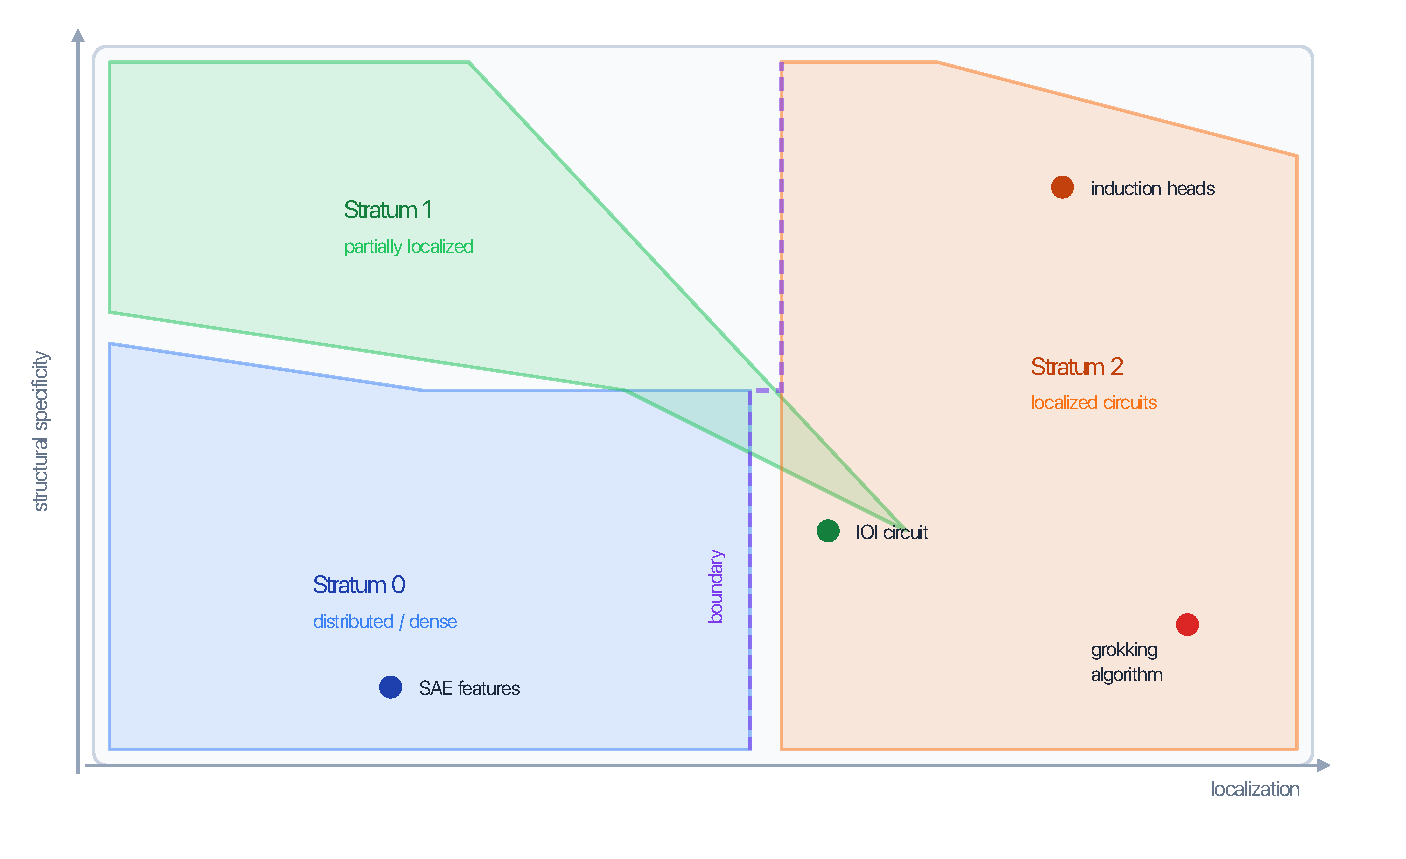
\includegraphics[width=\textwidth]{figures/strata-manifold.pdf}
\caption{Schematic of mechanism space as a stratified manifold.  Each stratum
  is a smoothly varying subset distinguished by the localization and structural
  specificity of the mechanism.  Boundaries between strata are lower-dimensional
  singular sets.  Empirical examples are placed roughly by the evidence reviewed
  in Section~\ref{sec:examples}; exact positions are schematic, not quantitative.}
\label{fig:strata}
\end{figure}

Figure~\ref{fig:strata} illustrates the key distinctions schematically.
The natural formalism is Whitney stratification \citep{whitney1965,golubitsky1973}:
a decomposition of mechanism space into smooth manifold strata that are
partially ordered by containment of their closures.  The stratified view
has a direct analogy in physics: the renormalization group (RG) describes
how the effective description of a system changes with measurement
resolution \citep{wilson1971,goldenfeld1992}.  RG fixed points correspond
to stable strata; relevant operators correspond to structure that survives
coarse-graining; universality classes correspond to mechanisms that appear
identical at a given resolution despite microscopic differences.  The
stratified view imports this resolution-dependence into interpretability.

A mechanism's stratum is determined
by its dimensionality, its localizability in specific components, and
the topology of its support in the residual stream.

\paragraph{Identity.}
Same stratum and same local equivalence class within the stratum.  Two
descriptions are the same mechanism if they name the same stratum and
agree on local structure within that stratum.

\paragraph{Evidence.}
Dimensionality tests (effective rank of the causal subspace),
localization diagnostics (is the mechanism's effect concentrated in a
small component set or distributed?), and stratum-transition tests
(does the apparent mechanism change stratum when the measurement
resolution changes?).

\paragraph{Failure modes.}
\emph{Stratum misidentification from method artifacts.}  A genuinely
distributed mechanism may appear localized to a single component if
the ablation method captures only the dominant direction.  Conversely,
a localized mechanism may appear distributed if the measurement method
has high background noise.  The stratified view does not resolve this
automatically---it provides the language to state it precisely.

\paragraph{Discriminating experiment.}
The stratified view predicts that measurement resolution affects the
apparent stratum.  Test this by comparing the effective dimensionality
of the causal subspace recovered by DAS at different hook points and
with different alignment constraints.  Consistent stratum across
resolutions supports a stratum assignment; stratum-change suggests
either a higher-stratum mechanism being partially recovered or a
measurement artifact.

\subsection{Perspectival View}

The perspectival view treats methods as revealing partial projections of
mechanisms rather than the mechanism in itself.  Disagreement between
methods is not automatically a failure; it may reveal the method-relative
structure of what is being measured.  This view is philosophically related
to Massimi's perspectival realism \citep{massimi2022}: the claim is not
that mechanisms are relative to methods (that would be instrumentalism),
but that scientific methods are partial perspectives on a
method-independent mechanistic structure.  The key distinction---between
perspectival \emph{evidence} (measurements are always from a vantage
point) and perspectival \emph{truth} (what's true depends on who measures
it)---maps directly onto the primary failure mode: conflating the
method-relativity of evidence with the claim that mechanisms are
themselves method-relative objects.

Identity is coherence across perspectives: two descriptions refer to the
same mechanism if they are mutually consistent and jointly interpretable
as projections of the same underlying structure.  Evidence is
multi-method robustness, formalized as
convergence across structural (weight), causal (activation/intervention),
and dynamic (training-time) evidence families.  The discriminating
experiment is cross-method consistency: test whether a patching-supported
claim is also supported by weight-space composition scores.  If not,
a third method adjudicates.

\subsection{Instrumental View}

The instrumental view treats mechanisms as useful predictive or
interventional models, warranted by forecast accuracy and intervention
utility regardless of whether they identify a real internal object.
Identity is predictive equivalence: two descriptions are the same
mechanism if they make the same predictions about all interventions and
behaviors.  This has the weakest ontological commitments and is therefore
the easiest to satisfy---but also the most limited.  The primary failure
mode is \emph{safety-relevant overreach}: claims that require strong
ontological conclusions (``the model is pursuing a goal'') cannot be
supported by predictive utility on the training distribution alone.
The discriminating experiment: test whether the mechanism label generates
novel predictions beyond the behavior used to identify it.

\subsection{Contrastive View}

The contrastive view treats mechanisms as defined relative to a foil:
a mechanism is what a component or subspace does in condition $A$
\emph{compared to} condition $B$.  This is how most interpretability
experiments actually work in practice---the IOI circuit is studied by
contrasting indirect-object completion with subject completion, not by
characterizing what heads do in absolute terms---but the contrastive
structure is rarely made explicit as an ontological commitment.

The contrastive view draws on a well-developed tradition in philosophy
of science.  Van Fraassen's pragmatic theory of explanation holds that
explanations are always contrastive: we explain why $P$ rather than $Q$,
not why $P$ simpliciter \citep{vanfraassen1980}.  Lipton's contrastive
epistemology extends this to inference: we infer the cause of $P$-rather-than-$Q$,
and different foils can yield different (and jointly correct) causal
explanations \citep{lipton1990}.

\paragraph{Identity.}
Two mechanism descriptions refer to the same mechanism iff they produce
the same contrastive pattern across the same foil set.  A ``name mover''
mechanism identified by contrasting IO with S tokens is a different
contrastive mechanism from one identified by contrasting IO tokens with
random tokens, even if both identify the same head---because the foil
determines what aspect of the head's behavior is being explained.

\paragraph{Evidence.}
Contrastive evidence requires specifying both the target condition and
the foil.  Activation patching with a specific counterfactual is
inherently contrastive (the counterfactual is the foil); mean ablation
is less so (the foil is an average, not a specific alternative).  The
strongest contrastive evidence comes from systematic variation of the
foil set: if the mechanism's effect is stable across foils within a
class but changes across foil classes, the contrastive boundary reveals
the mechanism's scope.

\paragraph{Failure modes.}
\emph{Foil dependence without acknowledgment}: reporting a mechanism
claim without specifying the foil, then treating it as an absolute
characterization.  \emph{Foil cherry-picking}: choosing the foil that
produces the cleanest result without testing alternatives.

\paragraph{Discriminating experiment.}
Take a published mechanism claim and vary the foil systematically.  If
the circuit identified for IOI changes when the foil is changed from
``repeat the subject'' to ``output a random name'' to ``output nothing,''
the mechanism is foil-relative and should be stated as such.

\subsection{The Determination Chain}\label{sec:chain}

The five axes are not independent.  In practice, the relationship is
mostly a chain of determination:
\[
\text{Ontology} \;\longrightarrow\; \text{Identity} \;\longrightarrow\; \text{Formalism}
\]
Choosing what kind of thing a mechanism \emph{is} determines when two
mechanisms are the \emph{same}, which in turn determines what
\emph{mathematical structure} can express the claim.  If mechanisms are
causal subspaces, identity is geodesic proximity on $\Gr(k,d)$, and the
formalism must include Grassmannian geometry.  If mechanisms are
gauge-invariant structures, identity is gauge-orbit membership, and the
formalism must include fiber bundles and holonomy groups.  The chain is
mostly one-to-one: each of the nine ontological commitments in the atlas
implies a specific identity criterion, which implies a specific ambient
formalism (Table~\ref{tab:atlas}).

Evidence and target are constrained by the ontology--identity pair but
not fully determined by it: a subspace claim can be supported by
activation-space evidence (DAS), weight-space evidence (SVD), or both,
and the target is chosen by the researcher.  The determination chain
therefore has two free parameters once the ontology is fixed.

This structure explains why the most common coherence violations involve
mismatches between the first three axes: using a subspace formalism
(Grassmannian distance) while holding an object ontology (component
overlap identity), or using an object evidence type (activation patching)
to support a structural claim (gauge-orbit identity).  The chain makes
these mismatches visible.

\subsection{View Families and Ontological Commitment}\label{sec:families}

The nine views group into families based on their shared structure
(Figure~\ref{fig:families}):

\begin{itemize}[leftmargin=*]
\item \textbf{Identity family} (Object, Role): mechanisms are identified
      by what they are (components) or what they do (functions).  Lowest
      mathematical overhead; most of the current literature operates here.
\item \textbf{Mathematical family} (Subspace, Structural): mechanisms
      live in geometric spaces and identity is defined by distances or
      orbits in those spaces.  Requires differential geometry.
\item \textbf{Process family} (Process, Stratified): mechanisms are
      temporally extended or resolution-dependent.  Requires dynamical
      systems theory or stratification theory.
\item \textbf{Methodological singleton} (Perspectival): no single
      method reveals the mechanism; identity requires cross-method
      coherence.
\item \textbf{Pragmatic singleton} (Instrumental): mechanisms are useful
      models; identity is predictive equivalence.
\item \textbf{Contrastive singleton} (Contrastive): mechanisms are
      defined relative to a foil; identity requires matching contrastive
      patterns.
\end{itemize}

One natural (though not unique) ordering of the views is by
increasing ontological commitment---how much they claim about the
existence and nature of the mechanism independent of any measurement
procedure:
\[
\text{Instrumental} \;<\; \text{Contrastive} \;<\; \text{Perspectival}
\;<\; \text{Object} \;<\; \text{Role} \;<\; \text{Subspace} \;<\;
\text{Structural} \;<\; \text{Process} \;<\; \text{Stratified}
\]
This ordering is approximate: one could argue that Role has less
ontological commitment than Object (since a role is multiply realizable
while a component identity is tied to a specific model), and the
relative positions of Process and Structural depend on whether one
weights temporal or algebraic structure as ``more committed.''  What is
clear is the endpoints: the instrumental view requires only predictive
utility, while the stratified view requires evidence across multiple
strata and measurement resolutions.  Most published interpretability
work operates at the Object or Role level.  Moving to
higher-commitment views requires explicitly stating which view is
operative and supplying the corresponding evidence.

\begin{figure}[H]
\centering
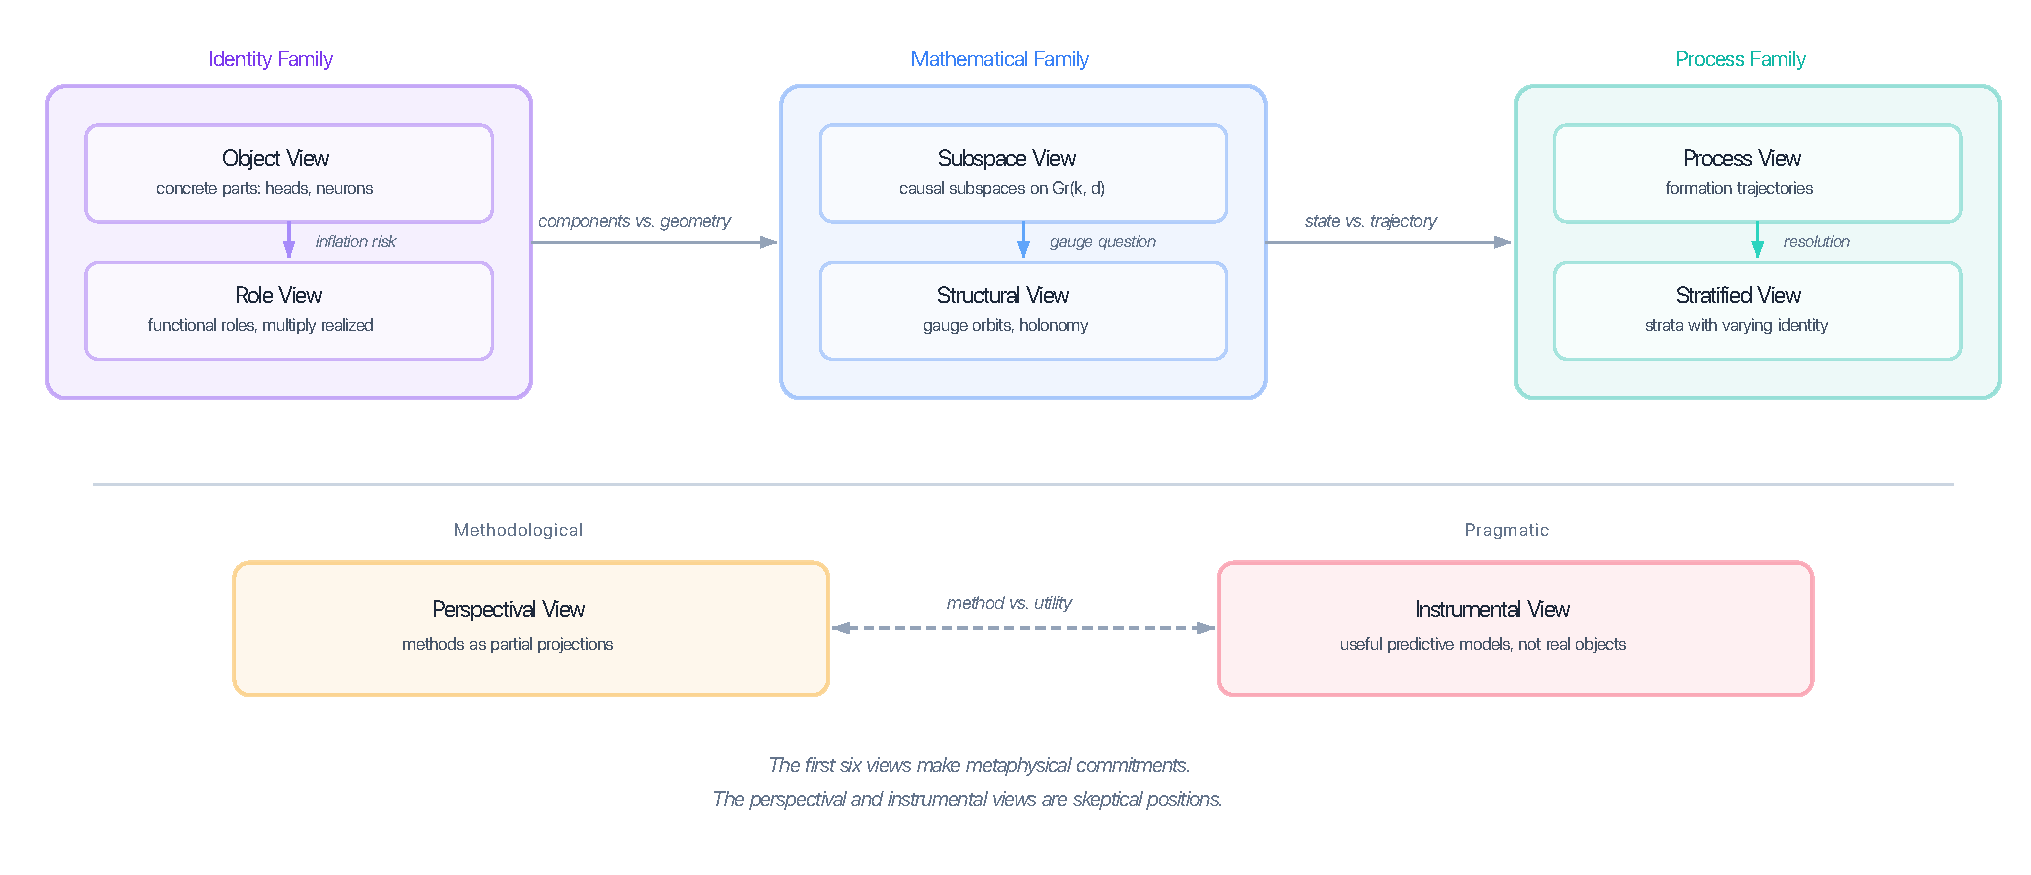
\includegraphics[width=\textwidth]{figures/eight-views-families.pdf}
\caption{The nine views grouped into three families (identity, mathematical,
  process) plus three singletons (methodological, pragmatic, contrastive),
  ordered by increasing ontological commitment.  Within each family, the
  internal arrow marks the principal decision point between the two views.}
\label{fig:families}
\end{figure}

\begin{figure}[H]
\centering
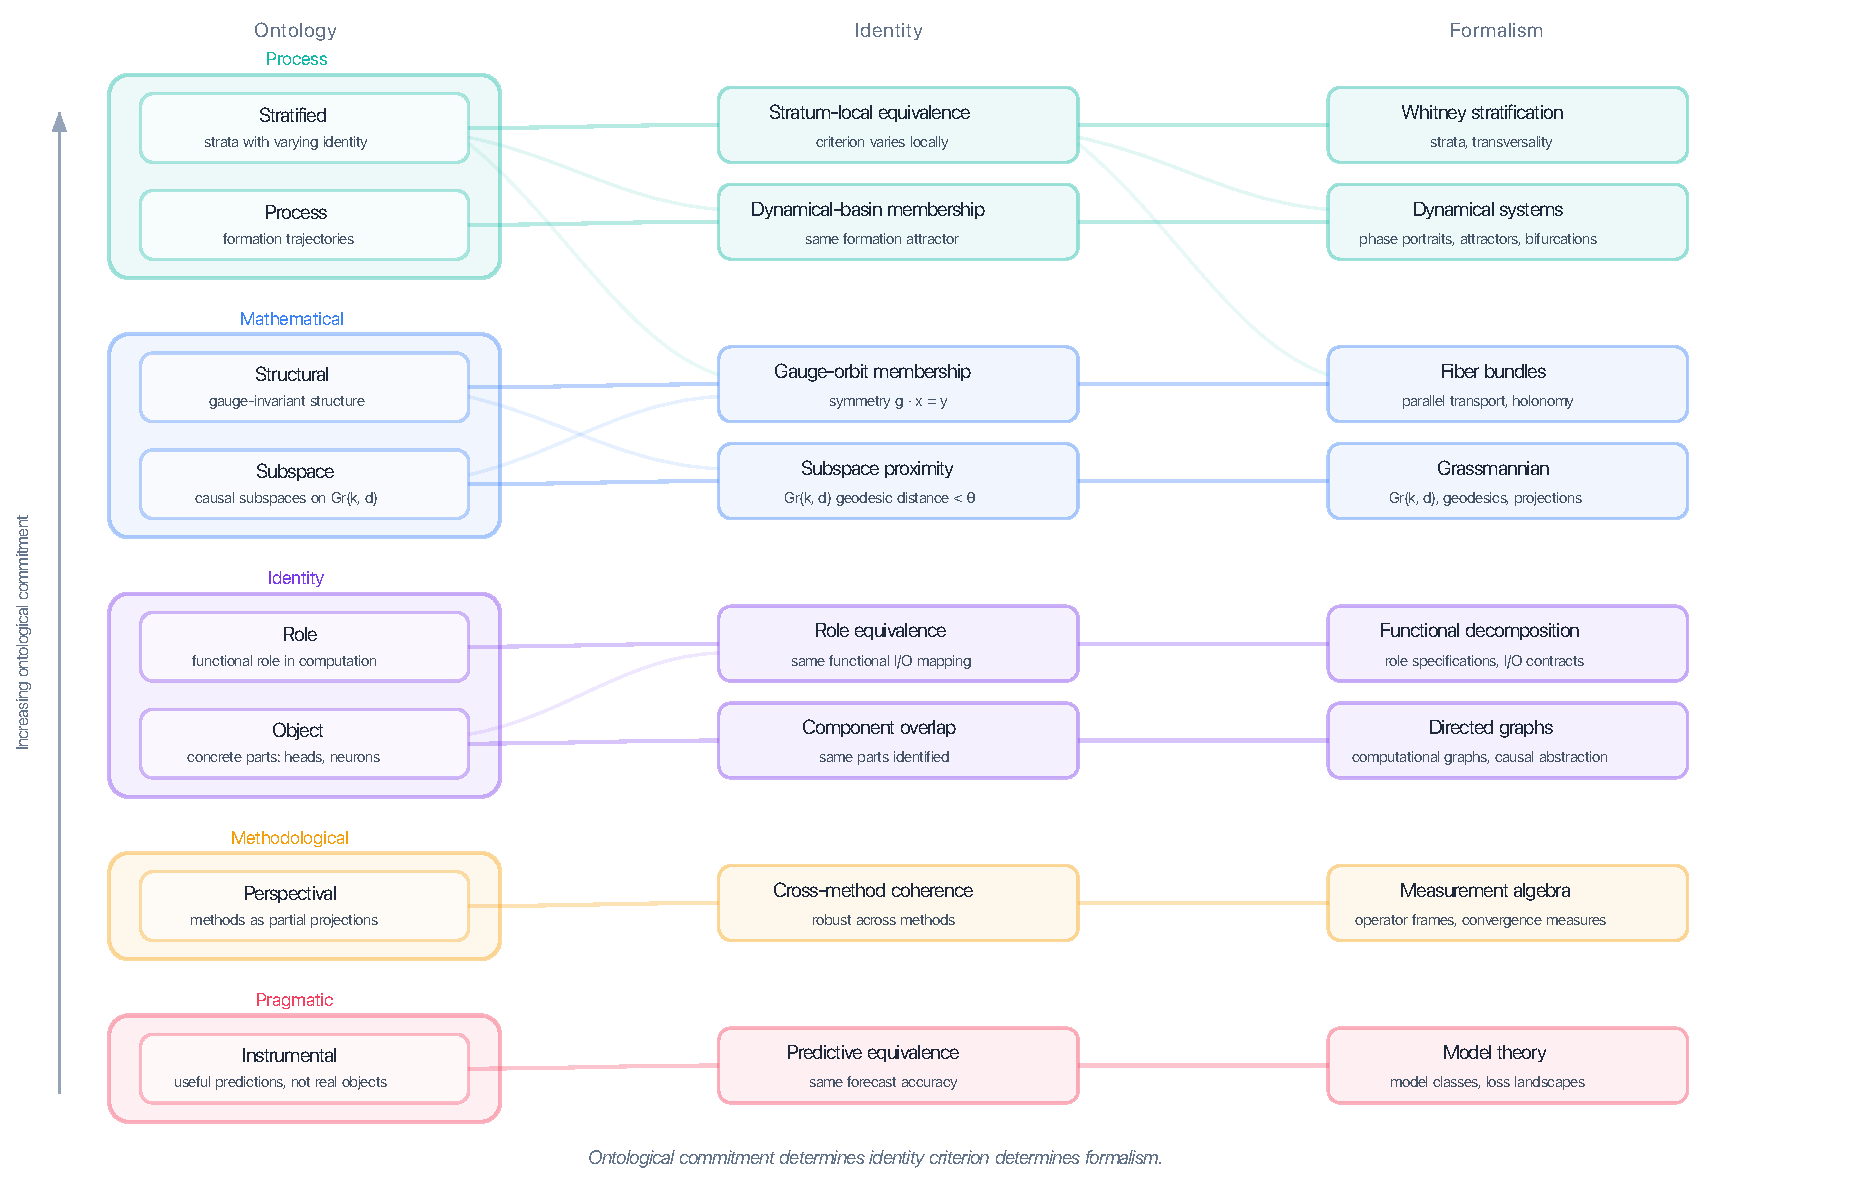
\includegraphics[width=\textwidth]{figures/ontology-identity-formalism.pdf}
\caption{The determination chain: ontology determines identity determines
  formalism.  Each view's ontological commitment (left) implies a specific
  identity criterion (center), which implies a natural mathematical formalism
  (right).  Primary connections are shown in bold; secondary cross-connections
  are shown faintly.  Increasing ontological commitment runs from bottom
  to top.}
\label{fig:determination}
\end{figure}

\subsection{Methods Mapping}\label{sec:methods}

Each commonly used interpretability method carries implicit commitments
across all five axes.  Table~\ref{tab:methods} makes these explicit.

\begin{table}[H]
\centering
\small
\setlength{\tabcolsep}{3.5pt}
\begin{tabular}{p{0.15\linewidth}p{0.11\linewidth}p{0.14\linewidth}p{0.14\linewidth}p{0.16\linewidth}p{0.14\linewidth}}
\toprule
\textbf{Method} & \textbf{Ontology} & \textbf{Identity} & \textbf{Evidence} & \textbf{Formalism} & \textbf{Target} \\
\midrule
Activation patching & Object & Component overlap & Activations & Directed graph & Task circuit \\[2pt]
Path patching       & Object & Component overlap & Activations & Directed graph & Task circuit \\[2pt]
ACDC                & Object & Component overlap & Activations & Directed graph & Task circuit \\[2pt]
EAP                 & Object & Component overlap & Act.\ + Wt. & Directed graph & Task circuit \\[2pt]
Ablation            & Object & Component overlap & Activations & Directed graph & Importance \\[2pt]
DAS / IIA           & Role$^\dagger$   & Role equivalence  & Activations & Subspace (borrowed) & Concept \\[2pt]
Causal scrubbing    & Role   & Role equivalence  & Activations & Causal graph & Alignment \\[2pt]
Linear probing      & Role   & Role equivalence  & Activations & Linear classifier & Detection \\[2pt]
SAE features        & Object & Component overlap & Activations & Dictionary & Feature catalog \\[2pt]
Logit / tuned lens  & Object & Component overlap & Activations & Linear proj. & Layer readout \\[2pt]
SVD of weights      & Subspace & Subspace prox. & Weights & $\Gr(k,d)$ & Decomposition \\[2pt]
Composition scores  & Structural & Gauge orbit  & Weights & Fiber bundle & Info-flow bound \\[2pt]
AGOP                & Process & Basin membership  & Dynamics & Dynamical sys. & Trajectory \\
\bottomrule
\end{tabular}
\caption{Five-axis classification of common interpretability methods.  Most
  methods are Object view with activation evidence.
  $^\dagger$DAS uses a subspace \emph{parameterization} (the alignment
  matrix searches over $\Gr(k,d)$) but Role \emph{identity}: it
  validates by IIA success, not Grassmannian distance.  The ontology is
  a hybrid---subspace search space, role validation criterion.}
\label{tab:methods}
\end{table}

Several patterns are visible.  First, the field's default operating point
is Object ontology with activation evidence: activation patching, path
patching, ACDC, ablation, SAE features, and logit lens all sit here.
Second, DAS occupies an interesting intermediate position: it uses a
subspace parameterization (the alignment matrix $Q$ searches over
subspaces) but validates by interchange intervention accuracy, which is a
\emph{role}-level criterion---whether two representations can be swapped
without loss of function.  The subspace is the search space, not the
ontology.  Third, no widely-used method operates in the Stratified or
Perspectival views---these views generate research programs rather than
describing current practice.

%% ---------------------------------------------------------------
\section{Worked Examples}\label{sec:examples}
%% ---------------------------------------------------------------

Three extended examples show what the atlas does in practice: not just
describing views in the abstract, but showing how the same body of
evidence is read differently under different views and what each reading
implies for follow-up work.  IOI illustrates a coherence violation
(the object-to-role slide); induction heads illustrate what convergence
across views looks like (the existence proof that the framework's
triangulation requirement is satisfiable); and superposition illustrates
the framework's strongest capacity---dissolving an active debate by
showing it is a view disagreement rather than an empirical one.
Additional case studies (SAE features, gender bias, factual recall,
hallucination, grokking, and others) appear in
Appendix~\ref{app:case_studies}.

\subsection{Indirect Object Identification}

\citet{wang2022} identify a circuit for indirect object identification
(IOI) in GPT-2 Small: 26 attention heads organized into functional
classes including S-inhibition heads, name movers, and
duplicate-token detection heads.

\paragraph{Object view.}
The mechanism is those 26 heads.  The evidence (activation and path
patching, mean ablation) establishes causal necessity and sufficiency
relative to the test distribution.  Object-level identity is precise
within GPT-2 Small and fails across architectures.

The object-level result is solid.  What it does not establish: (a) that
these heads perform a functional role that would be recognizable in
another model, (b) that the relevant causal variables are localized in
specific subspaces, (c) that the result is invariant under parameter
reparameterizations, or (d) how the circuit formed.  Claims (a)--(d)
require distinct evidence.

\paragraph{Role view.}
The four role classes (S-inhibition, name mover, duplicate-token
detection, and backup name mover) constitute a role-level description.
This is a hypothesis about what the heads do, not a confirmed role claim.
To confirm it, each role should be operationalized and tested
independently: name movers should copy tokens in novel syntactic
constructions; S-inhibition heads should suppress the subject in novel
contexts where the subject--object relationship is structurally varied.
Until these tests are run, the role labels describe the experimental
template more than the mechanism.

\paragraph{Subspace view.}
The subspace question is where the IO and S tokens, and the inhibitory
relationship between them, are represented in the residual stream.
DAS with linear alignment constraints would identify the causal
subspaces for each variable and test whether they can be independently
intervened on.  The 26-head object-level description does not resolve
this: two different subspace configurations could produce the same
patching results.

\paragraph{Structural view.}
The structural question is which aspects of the circuit are
gauge-invariant.  Path-patching results that survive
computation-preserving reparameterizations of the relevant head weights
establish structural facts; those that do not are basis-dependent
observations.  The holonomy of the circuit's transport map would provide
a structural fingerprint that is invariant across model instances.

\paragraph{Contrastive view.}
The IOI circuit is inherently contrastive: it characterizes what heads
do when distinguishing the indirect object from the subject.  A
different foil---IO vs.\ random token, or IO vs.\ nothing---would
identify a different contrastive mechanism, possibly with different
component involvement.  \citet{franco2026} confirm this: ABBA and BABA
prompt templates, which instantiate different foil structures, activate
different circuit topologies within the same model.

\paragraph{Verdicts.}
\emph{Object view}: the object-level claim is established; the 26-head
circuit is causally necessary on the test distribution.
\emph{Role view}: role identity is asserted, not confirmed; no
independent role operationalization exists.
\emph{Subspace view}: not attempted; the causal subspaces have not been
identified.
\emph{Structural view}: not attempted; gauge invariance has not been
tested.
\emph{Contrastive view}: the IOI circuit as stated is foil-relative;
varying the foil changes the circuit.

\subsection{Induction Heads}

The induction head result \citep{olsson2022} is unusually well-supported,
precisely because multiple views converge on the same object.

\paragraph{Object view.}
Induction heads are identified by activation patching.  Their distinctive
attention pattern---attending to the token immediately after the previous
occurrence of the current token---is established across a large family
of transformers.  Object-level identity is extended cross-model by
demonstrating the pattern holds across model sizes and architectures.

\paragraph{Role view.}
The induction pattern defines a functional role that is operationalized
(it can be tested on any sequence with a repeated token) and confirmed
across model families.  This is one of the few cases in the literature
where role identity is genuinely established rather than hypothesized.
The role specification is independent of the component: any head that
attends to $t_{j}$ from position $i$ when token $t_i = t_{j-1}$ is an
induction head, regardless of layer or position.

\paragraph{Process view.}
The formation dynamics are studied across training checkpoints.  A
phase transition is identified at a specific step in the loss curve,
and the composition score between the head and its prefix-matching
partner increases sharply at that step \citep{olsson2022}.  This is
process-level evidence---it concerns how the mechanism formed, not
what it is at the final checkpoint.  The formation process is argued
to be causally responsible for the in-context learning capacity of the
model, a claim that requires process evidence precisely because it is
about the training-time origin of a behavior.

\paragraph{What remains open.}
Under the stratified view: induction heads appear to be point-localized
objects, but whether the relevant causal variable is localized to a
one-dimensional subspace (object stratum) or spans a small-dimensional
subspace is not established.  Under the structural view: the holonomy
of the induction head transport map has not been characterized.  Under
the subspace view: the exact subspace of the residual stream encoding
the ``previous occurrence'' variable and the ``current token'' variable
has not been jointly identified via DAS.

\paragraph{Verdicts.}
\emph{Object view}: established across model families.
\emph{Role view}: confirmed---one of the few cases where role identity
is genuinely operationalized and independently tested.
\emph{Process view}: established via checkpoint analysis and composition
score evolution.
\emph{Subspace and structural views}: not attempted.
The convergence across object, role, and process views is why the
induction head result can support relatively strong claims---it is the
existence proof that the framework's triangulation requirement is
satisfiable.  The gaps in subspace and structural evidence are where
further work would strengthen or qualify those claims.

\subsection{Superposition}
\label{sec:worked-superposition}

The hypothesis that neural networks represent more features than they have dimensions---\emph{superposition}---has become one of the central organizing problems in mechanistic interpretability \citep{elhage2022superposition}. Substantial engineering effort has been directed at ``solving'' superposition, primarily through sparse autoencoders (SAEs) that project activations into higher-dimensional spaces where features are disentangled \citep{bricken2023, templeton2024}. But whether superposition is a \emph{problem to be solved} depends on which mechanistic view one adopts. The framework reveals that the field's framing presupposes an ontological commitment that is rarely stated and never defended.

\paragraph{Object view.}
Under the Object view, features are discrete, countable parts of the model's representation. Superposition occurs when these parts are ``compressed'' into fewer dimensions than there are features, entangling them in the activation space. SAEs exist precisely to undo this compression: by training a wide autoencoder with a sparsity penalty, one recovers a dictionary of monosemantic units, each corresponding to a single feature \citep{bricken2023}. The implicit assumption is that a clean decomposition exists underneath the entanglement.

This framing encounters a difficulty it lacks the internal resources to resolve. Different SAE widths yield different feature sets: a $4\times$-width SAE finds features that a $16\times$-width SAE splits further, and a $64\times$-width SAE splits further still \citep{templeton2024}. Which width gives the ``right'' features? The Object view requires a determinate inventory of parts, but the inventory changes with the magnifying glass. No principled criterion within the view selects a canonical width.

\paragraph{Subspace view.}
The Subspace view reframes features as subspaces rather than individual directions. Superposition is not a compression artifact but a geometric property: subspaces can overlap, and in high-dimensional spaces, approximate orthogonality is abundant enough that substantial overlap is expected rather than pathological. The question shifts from ``how do we disentangle features?'' to ``how much do representational subspaces interfere, and does that interference degrade downstream computation?''

This reframing makes the SAE width problem dissolve into a measurable quantity. Different SAE widths correspond to different granularities of subspace decomposition, and the relationship between them can be characterized by Grassmannian distances between the recovered subspaces across widths and random seeds. If subspaces converge, they identify robust geometric structure; if they fragment, the decomposition at that granularity is an artifact.

\paragraph{Structural view.}
The Structural view offers the deepest reframe. If mechanistic structure is constituted by computational relationships rather than any particular parameterization, then superposition is a \emph{gauge choice}: a consequence of the coordinate system in which we inspect the model, not an intrinsic property of the computation. Two models with different superposition patterns may implement identical input-output mappings and preserve identical computational invariants. What matters structurally is not the degree of superposition but what computation is invariant under changes of basis.

\paragraph{Perspectival view.}
The claim ``neural networks are in superposition'' presupposes that there exist discrete features being compressed into fewer dimensions---but this is the Object view's ontology imposed as a universal empirical assumption. The canonical demonstration of superposition \citep{elhage2022superposition} uses toy models trained to reconstruct sparse, known input features. In that setting, superposition is rigorously defined because the ground-truth features are specified by construction. But large language models were not trained to reconstruct a sparse feature dictionary; they were trained to predict tokens. The mapping from the toy setting to real networks requires the assumption that LM representations decompose into sparse discrete features in the first place---precisely the assumption that is under investigation.

The Perspectival view flags this as a circularity risk: SAEs are trained with a sparsity prior that \emph{enforces} decomposition into discrete units, then the resulting dictionaries are taken as evidence that discrete features exist \citep{leask2025}. This does not mean SAEs are uninformative, but it means the evidence they provide for the superposition hypothesis is weaker than typically assumed.

\paragraph{Verdicts.}
\emph{Object view}: superposition is real and must be solved, but the decomposition is \emph{underdetermined}---no principled criterion selects the correct SAE width.
\emph{Subspace view}: superposition is \emph{testable geometry}---measure Grassmannian distances across widths and seeds to determine which subspaces are robust.
\emph{Structural view}: superposition is a \emph{gauge choice}---the productive question is what computation is invariant under reparameterization.
\emph{Perspectival view}: the claim that models ``are in superposition'' is \emph{theory-laden}---it imports the Object view's ontology as an unstated assumption, supported by toy models whose training objective differs from that of real language models.
The field's substantial investment in ``solving superposition'' is coherent under the Object view, but it assumes that view is correct---an assumption that is rarely stated and never defended.

%% ---------------------------------------------------------------
\section{Six Decision Points}\label{sec:decisions}
%% ---------------------------------------------------------------

Six recurring forks in empirical interpretability work change in
meaning depending on which view is operative.  We examine what each
view implies for each fork and, where views make conflicting predictions,
what evidence would adjudicate.

\subsection{Localized vs.\ Distributed}

The question is whether a mechanism is implemented by a small, specific
set of components or spread across many.

Under the \emph{object view}, this is an empirical question: which
minimal component set is causally necessary and sufficient?  Under
the \emph{subspace view}, it is about the dimensionality and
localizability of the causal subspace: a low-rank subspace localized
in a small number of attention heads is one answer; a high-dimensional
subspace spanning many heads is another.  Under the \emph{stratified
view}, it is a question about which stratum the evidence supports.

The views come apart in practice.  Activation patching may identify a
small object-level component set as causally necessary, while DAS
identifies a high-dimensional subspace spanning many components.  These
need not be contradictory: the patching identifies the components whose
activation values lie in the relevant subspace; DAS characterizes the
subspace.  The stratified view provides the language to say that the
two results are compatible descriptions at different levels of
resolution.

\subsection{Object vs.\ Role}

The question is whether a mechanism claim is about a specific component
or about a functional role that component plays.  Under the \emph{object
view}, the claim is about the component; under the \emph{role view},
it is about the function.

The distinction matters for generalization.  An object claim does not
entail that any component in any other model is the same mechanism.  A
role claim does---if the role is operationalized and tested.  A common pattern is to establish object identity and then introduce a
role label in the same passage (``head 9.9, which we call a name
mover, ...''): the object identity is established, and the role label
is natural shorthand, but it carries additional commitments that the
object evidence alone does not discharge.

\subsection{Single vs.\ Triangulated Evidence}

The question is whether a mechanistic claim requires evidence from a
single method or convergent evidence from multiple methods with
independent assumptions.

Under the \emph{object view} with activation patching, a single strong
patching result may be sufficient.  Under the \emph{subspace view},
weight-space and activation-space convergence strengthens the claim
(both should identify the same subspace if the view is correct).
Under the \emph{perspectival view}, single-method evidence is always
vulnerable to that method's confounds: triangulation is definitionally
required.

The case for triangulation is not merely a caution.  If a method $m$
can only support claims in its range $C(m)$, and the target claim is
not in $C(m)$, then no amount of evidence from $m$ can support the
claim---however strong that evidence is.

\subsection{Static vs.\ Process}

The question is whether the mechanism is a final-checkpoint artifact
or a formation process.  This is a clean view-level distinction with
a clean evidential consequence: process claims need process evidence;
checkpoint claims cannot support process conclusions.

This matters most for: (a) training-dynamics hypotheses (``the model
learned to do $X$ because ...''), (b) phase-transition-like generalization
patterns, and (c) claims about the origin of in-context learning
behaviors.  In all three cases, checkpoint evidence establishes what
the mechanism is at convergence but not how it came to be.

\subsection{Subspace vs.\ Structural}

The question is whether mechanism identity is determined by the subspace
a mechanism occupies or by the gauge-invariant structure of the
computation it performs.  A subspace claim is basis-invariant: the
subspace $\mathrm{span}(Q)$ is the same regardless of which orthonormal
basis of $Q$ is used.  But it is not symmetry-invariant: two subspace
mechanisms in the same gauge orbit (related by a computation-preserving
symmetry that rotates the subspace) would be the same mechanism under
the structural view but potentially different under the subspace view.

The structural view is more realist and harder to operationalize.  The
subspace view is more tractable and directly supported by current DAS
methodology.  For most practical questions in the field, the subspace
view is appropriate; the structural view becomes important when
comparing across parameterizations of the same architecture or when
making claims that should be invariant to training randomness.

\subsection{Behavioral vs.\ Mechanistic}

The question is whether a finding is about a model's \emph{behavioral
propensity} (how it tends to behave on a distribution) or about a
\emph{mechanism} (an internal structure that produces behavior).
\citet{steinhardt2026} argues---in the context of evaluation
methodology, not ontology---that the field over-invests in capability
evaluation (can the model do~$X$?) and under-invests in propensity
evaluation (does the model typically do~$X$, and under what conditions?).
The distinction is relevant here because different views assign
different status to behavioral findings.

Under the \emph{instrumental view}, a behavioral finding---the model
reliably outputs~$Y$ given~$X$---is sufficient.  A propensity is what
you care about, and a mechanism is irrelevant.  Under the \emph{object
view}, a behavioral finding is a starting point: the question becomes
which components produce that behavior, and whether they are
necessary.  A capability finding (the model \emph{can} do~$X$) is
weaker than a propensity finding (the model \emph{typically does}~$X$)
because the former requires only that the relevant mechanism exists,
while the latter requires that it be routinely recruited.

The distinction matters most for safety.  A steering vector that
suppresses refusal behavior on a test distribution establishes an
instrumental capability---not a mechanistic understanding of
refusal~\citep{turner2024}.  Whether that vector \emph{is} the refusal
mechanism, or merely interferes with it, requires at least object-view
evidence (ablation of specific components) and ideally subspace-view
evidence (stability of the intervention direction across distributions).
The gap between instrumental evidence and the safety conclusions drawn
from it is the central evidence deficit identified by the open-problems
analysis in Appendix~\ref{app:openprobs}.


%% ---------------------------------------------------------------
\section{Using the Framework}\label{sec:implications}
%% ---------------------------------------------------------------

\subsection{The View Declaration Template}

The primary practical implication of this paper is that mechanistic
interpretability claims should state the view under which they are made.
We propose a five-line \emph{view declaration} that a paper would
include in its methods section:

\begin{quote}
\small
\textbf{View declaration.}
\emph{Ontology}: [what kind of entity counts as a mechanism].
\emph{Identity}: [when two descriptions refer to the same mechanism].
\emph{Evidence}: [what measurements support the claim].
\emph{Formalism}: [what mathematical language is used].
\emph{Target}: [what phenomenon is being explained].
\end{quote}

For example, the IOI circuit paper \citep{wang2022} would declare:

\begin{quote}
\small
\textbf{View declaration.}
\emph{Ontology}: concrete attention heads (Object view).
\emph{Identity}: component overlap within GPT-2 Small.
\emph{Evidence}: activation patching, path patching, mean ablation.
\emph{Formalism}: directed graph over 26 heads.
\emph{Target}: indirect object identification on the IOI distribution.
\end{quote}

This is not bureaucratic overhead---it is a precision requirement of
the same kind as reporting which distribution patching was run on.
Stating the view makes evidence-claim mismatches immediately visible:
if a paper declares Object ontology but draws Role conclusions
(``head~9.9 is a name mover''), the gap between the declared evidence
and the stated claim becomes a checkable coherence condition rather
than an unstated assumption.

\subsection{Common Coherence Violations}

Table~\ref{tab:violations} lists the five most common patterns
in which the evidence type and the claim type are mismatched.
Each row diagnoses the violation and identifies the evidence that
would resolve it.

\begin{table}[H]
\centering
\small
\begin{tabular}{p{0.20\linewidth}p{0.35\linewidth}p{0.35\linewidth}}
\toprule
\textbf{Violation} & \textbf{What it looks like} & \textbf{What would fix it} \\
\midrule
Object evidence, Role claim
  & ``Head~$X$ is a name mover'' (ablation only)
  & Role-specific prediction test on held-out constructions \\[4pt]
Unconstrained DAS
  & ``87\% IIA'' without specifying alignment class
  & State alignment class; rerun with linear constraint \citep{sutter2025} \\[4pt]
Object claim, Structural conclusion
  & ``Circuit is robust to fine-tuning''
  & Reparameterization stability test \\[4pt]
Process claim, no checkpoint evidence
  & ``Mechanism formed via phase transition''
  & Report composition score evolution across checkpoints \\[4pt]
Contrastive mechanism stated absolutely
  & ``The bias circuit encodes gender''
  & Report foil set; vary foil systematically \\
\bottomrule
\end{tabular}
\caption{Five common coherence violations and their resolutions.}
\label{tab:violations}
\end{table}

\subsection{Independent Convergence}

\citet{williams2025} argue from philosophy of science that MI needs
philosophical foundations---for clarifying concepts, refining methods,
and navigating epistemic complexity.  Their three central examples
(decomposition identity, feature ontology, deception detection) map
directly onto view-level analyses in this paper: ``no single correct
decomposition'' corresponds to the object--subspace distinction
(Section~\ref{sec:axes}); ``vehicle vs.\ content'' corresponds to the
object--role split applied to features; and ``behavioral detection is
insufficient for deception'' corresponds to the instrumental view's
ceiling (Appendix~\ref{app:openprobs}).  The convergence from
independent starting points---philosophy of science vs.\ measurement
theory---strengthens both analyses.

\subsection{Views as Research Programs}

The object and role views primarily organize existing empirical
practice.  The subspace, structural, and stratified views generate
positive research programs: each calls for methods, results, and
formalism that do not yet exist.  For the subspace view: systematic
DAS studies with stability tests across models and distributions.  For
the structural view: holonomy measurements, gauge-invariance checks,
and the development of geometric formalism.  For the stratified view:
dimensionality diagnostics and stratum-transition tests.  The atlas is
therefore not merely a taxonomy of current practice; it is a map of
what is missing.

%% ---------------------------------------------------------------
\section{Cross-View Promotion}\label{sec:promotion}
%% ---------------------------------------------------------------

\paragraph{Promotion conditions.}
A common question is: under what conditions can a result at one view be
promoted to a higher-commitment view?  The following are preliminary
promotion conditions:
\begin{itemize}[leftmargin=*]
\item \textbf{Object $\to$ Role.}  The component must be tested with an
      independently operationalized role specification on held-out
      constructions.  If the role predicts behavior beyond the original
      discovery distribution, the result can be stated as a role claim.
\item \textbf{Role $\to$ Subspace.}  The functional role must be shown to
      be mediated by a specific low-dimensional subspace (e.g., via linear
      DAS with linear alignment constraints), and this subspace must be stable
      across prompt distributions with small geodesic distance on $\Gr(k,d)$.
\item \textbf{Subspace $\to$ Structural.}  The subspace must survive
      computation-preserving symmetries of the weight space.  If the subspace
      recovered by DAS changes under a reparameterization that does not
      change the model's computation, the subspace claim is not structural.
      Holonomy measurements provide a gauge-invariant fingerprint.
\item \textbf{Any $\to$ Process.}  The static claim must be supplemented
      with training-dynamics evidence: checkpoint analysis showing when and
      how the mechanism formed, formation knockouts, or loss-curve structure.
      No amount of final-checkpoint evidence can substitute.
\end{itemize}
Each promotion requires new evidence of the kind specified by the target
view.  Evidence from the source view does not accumulate toward the
target view's standard---it answers a different question.  The chain is
not sequential: promotion can skip levels when the evidence supports it.
For example, an Object-level result can promote directly to Subspace if
linear DAS identifies a causal subspace spanning the relevant components,
without requiring an intermediate Role specification.  The subspace
evidence subsumes the object evidence (the components are where the
subspace has support) but does not require role-level mediation.

\paragraph{View selection: a practical heuristic.}
The framework is pluralist, but a researcher facing a concrete question
needs guidance on which view to adopt.  The following heuristic matches
the scope of the claim to the minimum view that can support it:
\begin{itemize}[leftmargin=*]
\item If the claim is about \emph{a specific model on a specific
      distribution}, the \textbf{Object view} is sufficient.
\item If the claim should \emph{generalize across models} (``Pythia and
      GPT-2 both have this mechanism''), at least the \textbf{Role view}
      is required---component indices are trivially not cross-model.
\item If the claim involves a \emph{distributed representation} not
      localized to a single component, the \textbf{Subspace view} is
      needed.
\item If the claim should \emph{survive reparameterization}
      (permutation, rescaling, rotation of weight matrices), the
      \textbf{Structural view} is needed.
\item If the claim is about \emph{how the mechanism formed} or why it
      appeared at a specific training step, the \textbf{Process view} is
      needed---no amount of checkpoint evidence can substitute.
\item If the mechanism's \emph{apparent type changes with measurement
      resolution}, the \textbf{Stratified view} is the appropriate
      language.
\end{itemize}
The heuristic is conservative: it recommends the lowest-commitment view
that matches the claim's scope.  Higher-commitment views are always
available but require correspondingly stronger evidence.

\paragraph{Connections to neighboring fields.}
The five-axis framework has natural translations into several disciplines
whose concepts it draws on.

\emph{Philosophy of science.}
The ontology axis corresponds to the central question of the new
mechanist literature: what counts as a mechanism
\citep{machamer2000,craver2007,illari2012,glennan1996}?  The identity
axis operationalizes the question that Lewis's account of functional
identification \citep{lewis1972} raises: under what conditions does a
mechanism remain ``the same''?  The
evidence axis inherits the eliminativist structure of Earman's Bayesian
epistemology \citep{earman1992} and the domain-triangulation principle
of Howson and Urbach \citep{howson1989}: independent evidence types
eliminate distinct confounders.  Massimi's perspectival realism
\citep{massimi2022} maps directly onto the perspectival view, with
the important distinction that perspectival evidence does not entail
perspectival truth.

\emph{Physics.}
The structural view's gauge-invariance requirement is the direct
analogue of gauge symmetry in field theory: two weight configurations
related by a computation-preserving transformation are physically
the same mechanism, just as two vector potentials related by a gauge
transformation describe the same electromagnetic field
\citep{nakahara2003}.  The stratified view borrows the renormalization
group's central insight \citep{wilson1971,goldenfeld1992}: effective
descriptions change with measurement scale, and the interesting
objects are the fixed points (stable strata) and relevant operators
(structure that survives coarse-graining).  Universality classes
in physics correspond to mechanisms that appear identical at a given
resolution despite differing microscopically.

\emph{Mathematics.}
The formalism axis is not merely notational.  The choice of
mathematical structure constrains what can be stated precisely and
what can be proved.  Grassmannian geometry \citep{nakahara2003}
makes subspace proximity a metric statement; fiber bundles make
gauge invariance a theorem rather than a heuristic check; Whitney
stratification \citep{whitney1965,golubitsky1973} gives a rigorous
account of how mechanism identity changes across strata boundaries.
Each formalism carries proof obligations that the corresponding
informal claim does not.

\emph{Cognitive science and neuroscience.}
The localization--distribution spectrum (object view through stratified
view) mirrors the longstanding debate between localizationism and
distributed coding in systems neuroscience
\citep{bechtel1993}.  The double dissociation methodology in
neuropsychology---showing two functions can be selectively impaired
independently---is the nearest analogue to the necessity and
sufficiency tests used in the object view.  Marr's tri-level account
\citep{marr1982} organizes explanatory targets; the five axes here
organize ontological commitments.  Both are needed, and they are
complementary: two researchers at the same Marr level can hold different
mechanistic views.

%% ---------------------------------------------------------------
\section{Open Questions}\label{sec:open}
%% ---------------------------------------------------------------

Several questions are raised by the framework and not resolved:
\begin{enumerate}[leftmargin=*]
\item \emph{Process identity.}  The identity criterion for the process
      view (same dynamical basin or trajectory type) is underspecified
      relative to the object, subspace, and structural criteria.
      Formalizing process identity is an open problem.
\item \emph{Cross-view promotion.}  Under what conditions can an
      object-level result be promoted to a subspace-level or structural-level
      result?  Section~\ref{sec:promotion} gives preliminary conditions, but
      a systematic account of inter-view inference is missing.
\item \emph{Completeness of the atlas.}  The nine views are identified
      by reading the literature, not derived from the five axes.  Whether
      there are important views not represented---a Marr computational-level
      view \citep{marr1982}, a representational-content view, a
      population-level statistical view---is an open question.
\item \emph{Sufficiency of the five axes.}  The five axes may be too many
      or too few.  Evidence and formalism are tightly constrained by
      ontology and identity (the determination chain), raising the question
      of whether they are genuinely free axes or downstream consequences.
      Conversely, the framework omits a normative dimension---it diagnoses
      coherence but not adequacy for a given purpose.  Whether adequacy
      is a sixth axis or a meta-level concern about the framework is open.
\item \emph{View-independence of the framework.}  The coherence
      conditions (\S\ref{sec:coherence}) assume crisp equivalence
      relations.  Both the Perspectival view (coherence across
      perspectives) and the Process view (dynamical basin membership)
      have inherently fuzzy identity criteria that may not satisfy
      transitivity.  Whether this is a limitation of the views or of
      the framework's formalization is unresolved.
\item \emph{Views and safety-relevant inference.}  Safety applications
      (monitoring, alignment auditing) require mechanistic claims that are
      robust to adversarial distribution shift.  What minimum view supports
      safety-relevant inference?  The object view is likely insufficient---a
      head identified as safety-relevant on one distribution may not
      generalize.  The structural or stratified views may be necessary, but
      their evidential demands are currently impractical at scale.
\item \emph{Implicit view commitments of existing programs.}  The
      monosemanticity program \citep{bricken2023,templeton2024} implicitly
      assumes that individual SAE dictionary elements are the right ontological
      unit (object view) with feature-level identity.  The causal abstraction
      program \citep{geiger2021,geiger2024} assumes role-level identity via
      interchange intervention.  Making these commitments explicit would
      clarify what each program can and cannot establish.
\end{enumerate}

%% ---------------------------------------------------------------
\section{Conclusion}
%% ---------------------------------------------------------------

Mechanistic interpretability is not only a search for circuits.  It is
a search for the right kind of object to call a mechanism.  The field
already uses multiple mechanistic views, typically implicitly, and making
those views explicit improves both the precision of claims and the
appropriateness of evidence.

The central contribution is a taxonomy: every mechanistic
interpretability result assumes a mechanistic view---a bundle of
commitments about ontology, identity, evidence, formalism, and
target---whether or not it is stated.  Coherence between these
components is not automatic (\S\ref{sec:coherence}), and the
determination chain---ontology constrains identity constrains
formalism---makes mismatches between them diagnosable.

The atlas of nine views---object, role, subspace, structural, process,
stratified, perspectival, instrumental, contrastive---covers the main
options currently in use or emerging.  Each view is appropriate for some
questions and inappropriate for others.  The paper is pluralist: the
goal is not to collapse this plurality into a master ontology but to
make view choice explicit, justifiable, and revisable.  The induction
head result remains the canonical illustration of what convergence
across views looks like: object, role, and process views all point to
the same entity, which is why the result supports claims that
single-view results cannot.

This paper addresses the ontological prerequisites for mechanistic
claims.  Companion work addresses the validity structure of individual
claims \citep{tower2026mechval}, the reference conditions for
cross-model identity \citep{tower2026mechref}, and the composition
conditions under which validated claims aggregate into system-level
understanding \citep{tower2026mechknow}.

%% ---------------------------------------------------------------
\bibliographystyle{plainnat}
\begin{thebibliography}{99}

\bibitem[Balesni et~al.(2024)]{apollo2024}
Mikita Balesni, Marius Hobbhahn, David Lindner, Alexander Meinke, Tomek
  Korbak, Joshua Clymer, Buck Shlegeris, Jeremy Scheurer, Charlotte Stix,
  et~al.
\newblock Towards evaluations-based safety cases for {AI} scheming.
\newblock arXiv:2411.03336, 2024.

\bibitem[Bechtel \& Richardson(1993)]{bechtel1993}
William Bechtel and Robert~C.\ Richardson.
\newblock \emph{Discovering Complexity: Decomposition and Localization as
  Strategies in Scientific Research}.
\newblock Princeton University Press, Princeton, NJ, 1993.

\bibitem[Bricken et~al.(2023)]{bricken2023}
Trenton Bricken, Adly Templeton, Joshua Batson, Brian Chen, Adam Jermyn,
  Tom Conerly, Nicholas L.\ Turner, Cem Anil, Carson Denison, Amanda Askell,
  Robert Lasenby, Yifan Wu, Shauna Kravec, Nicholas Schiefer, Tim Maxwell,
  Nicholas Joseph, Zac Hatfield-Dodds, Alex Tamkin, Karina Nguyen, Brayden
  McLean, Josiah E.\ Burke, Tristan Hume, Shan Carter, Tom Henighan, and
  Chris Olah.
\newblock Towards monosemanticity: Decomposing language models with dictionary
  learning.
\newblock \emph{Transformer Circuits Thread}, 2023.
\newblock \url{https://transformer-circuits.pub/2023/monosemanticity}.

\bibitem[Craver(2007)]{craver2007}
Carl F.\ Craver.
\newblock \emph{Explaining the Brain: Mechanisms and the Mosaic Unity of
  Neuroscience}.
\newblock Oxford University Press, Oxford, 2007.

\bibitem[Darden(2006)]{darden2006}
Lindley Darden.
\newblock \emph{Reasoning in Biological Discoveries: Essays on Mechanisms,
  Interfield Relations, and Anomaly Resolution}.
\newblock Cambridge University Press, Cambridge, 2006.

\bibitem[Earman(1992)]{earman1992}
John Earman.
\newblock \emph{Bayes or Bust? A Critical Examination of Bayesian Confirmation
  Theory}.
\newblock MIT Press, Cambridge, MA, 1992.

\bibitem[Elhage et~al.(2021)]{elhage2021}
Nelson Elhage, Neel Nanda, Catherine Olsson, Tom Henighan, Nicholas Joseph,
  Ben Mann, Amanda Askell, Yuntao Bai, Anna Chen, Tom Conerly, Nova DasSarma,
  Dawn Drain, Deep Ganguli, Zac Hatfield-Dodds, Danny Hernandez, Andy Jones,
  Jackson Kernion, Liane Lovitt, Kamal Ndousse, Dario Amodei, Tom Brown, Jack
  Clark, Jared Kaplan, Sam McCandlish, and Chris Olah.
\newblock A mathematical framework for transformer circuits.
\newblock \emph{Transformer Circuits Thread}, 2021.
\newblock \url{https://transformer-circuits.pub/2021/framework}.

\bibitem[Glennan(1996)]{glennan1996}
Stuart Glennan.
\newblock Mechanisms and the nature of causation.
\newblock \emph{Erkenntnis}, 44\penalty0 (1):\penalty0 49--71, 1996.

\bibitem[Geiger et~al.(2021)]{geiger2021}
Atticus Geiger, Hanson Lu, Thomas Icard, and Christopher Potts.
\newblock Causal abstractions of neural networks.
\newblock In \emph{Advances in Neural Information Processing Systems
  (NeurIPS)}, 2021.

\bibitem[Geiger et~al.(2024)]{geiger2024}
Atticus Geiger, Zhengxuan Wu, Christopher Potts, Thomas Icard, and Noah D.\
  Goodman.
\newblock Finding alignments between interpretable causal variables and
  distributed neural representations.
\newblock In \emph{Conference on Causal Learning and Reasoning (CLeaR)}, 2024.

\bibitem[Goldenfeld(1992)]{goldenfeld1992}
Nigel Goldenfeld.
\newblock \emph{Lectures on Phase Transitions and the Renormalization Group}.
\newblock Addison-Wesley, Reading, MA, 1992.

\bibitem[Golubitsky \& Guillemin(1973)]{golubitsky1973}
Martin Golubitsky and Victor Guillemin.
\newblock \emph{Stable Mappings and their Singularities}.
\newblock Springer-Verlag, New York, 1973.

\bibitem[Howson \& Urbach(1989)]{howson1989}
Colin Howson and Peter Urbach.
\newblock \emph{Scientific Reasoning: The Bayesian Approach}.
\newblock Open Court, La Salle, IL, 1989.

\bibitem[Illari \& Williamson(2012)]{illari2012}
Phyllis McKay Illari and Jon Williamson.
\newblock What is a mechanism? Thinking about mechanisms across the sciences.
\newblock \emph{European Journal for Philosophy of Science},
  2\penalty0 (1):\penalty0 119--135, 2012.

\bibitem[Machamer et~al.(2000)]{machamer2000}
Peter Machamer, Lindley Darden, and Carl F.\ Craver.
\newblock Thinking about mechanisms.
\newblock \emph{Philosophy of Science}, 67\penalty0 (1):\penalty0 1--25, 2000.

\bibitem[Lewis(1972)]{lewis1972}
David Lewis.
\newblock Psychophysical and theoretical identifications.
\newblock \emph{Australasian Journal of Philosophy}, 50(3):249--258, 1972.

\bibitem[Marr(1982)]{marr1982}
David Marr.
\newblock \emph{Vision: A Computational Investigation into the Human
  Representation and Processing of Visual Information}.
\newblock W.\ H.\ Freeman, San Francisco, 1982.

\bibitem[Massimi(2022)]{massimi2022}
Michela Massimi.
\newblock \emph{Perspectival Realism}.
\newblock Oxford University Press, Oxford, 2022.

\bibitem[Nakahara(2003)]{nakahara2003}
Mikio Nakahara.
\newblock \emph{Geometry, Topology and Physics}.
\newblock Institute of Physics Publishing, Bristol, 2nd edition, 2003.

\bibitem[MIB(2025)]{mib2025}
Mechanistic Interpretability Benchmark.
\newblock Comprehensive evaluation for circuit discovery methods.
\newblock 2025.
\newblock \url{https://github.com/mechanistic-interpretability-benchmark/mib}.

\bibitem[Merullo et~al.(2024)]{merullo2024}
Jack Merullo, Carsten Eickhoff, and Ellie Pavlick.
\newblock Talking heads: Understanding inter-layer communication in transformer
  language models.
\newblock arXiv:2406.09519, 2024.

\bibitem[Nanda(2022)]{nanda2022open}
Neel Nanda.
\newblock 200 concrete open problems in mechanistic interpretability.
\newblock Blog post, 2022.
\newblock \url{https://www.neelnanda.io/mechanistic-interpretability/200-open-problems}.

\bibitem[Ngo et~al.(2022)]{ngo2022}
Richard Ngo, Lawrence Chan, and S\"oren Mindermann.
\newblock The alignment problem from a deep learning perspective.
\newblock arXiv:2209.00626, 2022.

\bibitem[Olsson et~al.(2022)]{olsson2022}
Catherine Olsson, Nelson Elhage, Neel Nanda, Nicholas Joseph, Nova DasSarma,
  Tom Henighan, Ben Mann, Amanda Askell, Yuntao Bai, Anna Chen, et~al.
\newblock In-context learning and induction heads.
\newblock \emph{Transformer Circuits Thread}, 2022.
\newblock \url{https://transformer-circuits.pub/2022/in-context-learning-and-induction-heads}.

\bibitem[Schmidt Futures(2026)]{schmidt2026}
Schmidt Futures.
\newblock Trustworthy AI research agenda.
\newblock Request for proposals, 2026.

\bibitem[Sharkey et~al.(2025)]{sharkey2025}
Lee Sharkey, Bilal Chughtai, Joshua Batson, Jack Lindsey, Jeff Wu, Lucius
  Bushnaq, Nicholas Goldowsky-Dill, Stefan Heimersheim, et~al.
\newblock Open problems in mechanistic interpretability.
\newblock arXiv:2501.16496, 2025.

\bibitem[Quine(1948)]{quine1948}
Willard Van~Orman Quine.
\newblock On what there is.
\newblock \emph{Review of Metaphysics}, 2\penalty0 (5):\penalty0 21--38, 1948.

\bibitem[Steinhardt(2026)]{steinhardt2026}
Jacob Steinhardt.
\newblock The case for evaluating model behaviors.
\newblock Alignment Forum, May 2026.

\bibitem[Sutter et~al.(2025)]{sutter2025}
Denis Sutter, Julian Minder, Thomas Hofmann, and Tiago Pimentel.
\newblock The non-linear representation dilemma: Is causal abstraction enough
  for mechanistic interpretability?
\newblock In \emph{Advances in Neural Information Processing Systems
  (NeurIPS)}, 2025.

\bibitem[Templeton et~al.(2024)]{templeton2024}
Adly Templeton et~al.
\newblock Scaling monosemanticity: Extracting interpretable features from
  {Claude 3 Sonnet}.
\newblock \emph{Anthropic Transformer Circuits Thread}, 2024.
\newblock \url{https://transformer-circuits.pub/2024/scaling-monosemanticity}.

\bibitem[Turner et~al.(2024)]{turner2024}
Alex Turner, Lisa Thiergart, Gavin Leech, David Udell, Juan~J.\ Vazquez,
  Ulisse Mini, and Monte MacDiarmid.
\newblock Activation addition: Steering language models without optimization.
\newblock arXiv:2308.10248, 2024.

\bibitem[Wang et~al.(2022)]{wang2022}
Kevin Wang, Alexandre Variengien, Arthur Conmy, Buck Shlegeris, and Jacob
  Steinhardt.
\newblock Interpretability in the wild: A circuit for indirect object
  identification in {GPT-2 Small}.
\newblock arXiv:2211.00593, 2022.

\bibitem[van Fraassen(1980)]{vanfraassen1980}
Bas~C. van Fraassen.
\newblock \emph{The Scientific Image}.
\newblock Oxford University Press, Oxford, 1980.

\bibitem[Lipton(1990)]{lipton1990}
Peter Lipton.
\newblock Contrastive explanation.
\newblock \emph{Royal Institute of Philosophy Supplements}, 27:\penalty0
  247--266, 1990.

\bibitem[Williams et~al.(2025)]{williams2025}
Iwan Williams, Ninell Oldenburg, Ruchira Dhar, Joshua Hatherley, Constanza
  Fierro, Nina Rajcic, Sandrine~R.\ Schiller, Filippos Stamatiou, and Anders
  S{\o}gaard.
\newblock Mechanistic interpretability needs philosophy.
\newblock arXiv:2506.18852, 2025.

\bibitem[Whitney(1965)]{whitney1965}
Hassler Whitney.
\newblock Tangents to an analytic variety.
\newblock \emph{Annals of Mathematics}, 81\penalty0 (3):\penalty0 496--549, 1965.

\bibitem[Wilson(1971)]{wilson1971}
Kenneth G.\ Wilson.
\newblock Renormalization group and critical phenomena.\ {I}.\ Renormalization
  group and the {Kadanoff} scaling picture.
\newblock \emph{Physical Review B}, 4\penalty0 (9):\penalty0 3174--3183, 1971.

\bibitem[Tigges et~al.(2024)]{tigges2024}
Curt Tigges, Oskar John Hollinsworth, Atticus Geiger, and Neel Nanda.
\newblock {LLM} circuit analyses are consistent across training and scale.
\newblock arXiv:2407.10827, 2024.

\bibitem[Bali et~al.(2026)]{bali2026}
Karan Bali, Jack Stanley, Praneet Suresh, and Danilo Bzdok.
\newblock Quantifying {LLM} attention-head stability: Implications for circuit
  universality.
\newblock arXiv:2602.16740, 2026.

\bibitem[Franco et~al.(2026)]{franco2026}
Guilherme Franco, Lucas~M.\ Tassis, Achille Rohr, and Mark Crovella.
\newblock Finding highly interpretable prompt-specific circuits in language
  models.
\newblock arXiv:2602.13483, 2026.

\bibitem[Sun \& Toneva(2026)]{sun2026}
Alan Sun and Mariya Toneva.
\newblock Tracking equivalent mechanistic interpretations across neural
  networks.
\newblock In \emph{International Conference on Learning Representations
  (ICLR)}, 2026.

\bibitem[Leask et~al.(2025)]{leask2025}
Patrick Leask, Joshua Mendel, Maria Koumeri, Nenad Tomasev, Kenneth Li, and
  Wes Gurnee.
\newblock Sparse autoencoders do not find canonical units of computation.
\newblock In \emph{International Conference on Learning Representations
  (ICLR)}, 2025.

\bibitem[Tower(2026a)]{tower2026mechval}
Elliot Tower.
\newblock Mechanistic validation: Evidence standards for mechanism claims.
\newblock arXiv preprint, 2026.

\bibitem[Tower(2026b)]{tower2026mechref}
Elliot Tower.
\newblock Mechanistic reference: When does a mechanism term pick out the same
  thing?
\newblock arXiv preprint, 2026.

\bibitem[Tower(2026c)]{tower2026mechknow}
Elliot Tower.
\newblock When do circuit discoveries compose into understanding?
\newblock arXiv preprint, 2026.

\bibitem[Elhage et~al.(2022)]{elhage2022superposition}
Nelson Elhage, Tristan Hume, Catherine Olsson, Nicholas Schiefer, Tom Henighan,
  Shauna Kravec, Zac Hatfield-Dodds, Robert Lasenby, Dawn Drain, Carol Chen,
  et~al.
\newblock Toy models of superposition.
\newblock \emph{Transformer Circuits Thread}, 2022.

\bibitem[Bolukbasi et~al.(2016)]{bolukbasi2016}
Tolga Bolukbasi, Kai-Wei Chang, James Zou, Venkatesh Saligrama, and Adam Kalai.
\newblock Man is to computer programmer as woman is to homemaker? Debiasing word
  embeddings.
\newblock In \emph{Advances in Neural Information Processing Systems (NeurIPS)}, 2016.

\bibitem[Vig et~al.(2020)]{vig2020causal}
Jesse Vig, Sebastian Gehrmann, Yonatan Belinkov, Sharon Qian, Daniel Nevo,
  Yaron Singer, and Stuart Shieber.
\newblock Investigating gender bias in language models using causal mediation
  analysis.
\newblock In \emph{Advances in Neural Information Processing Systems (NeurIPS)}, 2020.

\bibitem[Li et~al.(2023a)]{li2023iti}
Kenneth Li, Oam Patel, Fernanda Vi\'{e}gas, Hanspeter Pfister, and Martin Wattenberg.
\newblock Inference-time intervention: Eliciting truthful answers from a
  language model.
\newblock In \emph{Advances in Neural Information Processing Systems (NeurIPS)}, 2023.

\bibitem[Meng et~al.(2022)]{meng2022}
Kevin Meng, David Bau, Alex Andonian, and Yonatan Belinkov.
\newblock Locating and editing factual associations in {GPT}.
\newblock In \emph{Advances in Neural Information Processing Systems (NeurIPS)}, 2022.

\bibitem[Power et~al.(2022)]{power2022grokking}
Alethea Power, Yuri Burda, Harri Edwards, Igor Babuschkin, and Vedant Misra.
\newblock Grokking: Generalization beyond overfitting on small algorithmic
  datasets.
\newblock arXiv:2201.02177, 2022.

\bibitem[Nanda et~al.(2023)]{nanda2023grokking}
Neel Nanda, Lawrence Chan, Tom Lieberum, Jess Smith, and Jacob Steinhardt.
\newblock Progress measures for grokking via mechanistic interpretability.
\newblock In \emph{International Conference on Learning Representations (ICLR)}, 2023.

\bibitem[Conmy et~al.(2023)]{conmy2023acdc}
Arthur Conmy, Augustine N.\ Mavor-Parker, Aengus Lynch, Stefan Heimersheim,
  and Adri\`{a} Garriga-Alonso.
\newblock Towards automated circuit discovery for mechanistic interpretability.
\newblock In \emph{Advances in Neural Information Processing Systems (NeurIPS)}, 2023.

\bibitem[Syed et~al.(2023)]{syed2023eap}
Aaquib Syed, Can Rager, and Arthur Conmy.
\newblock Attribution patching outperforms automated circuit discovery.
\newblock arXiv:2310.10348, 2023.

\bibitem[Lanham et~al.(2023)]{lanham2023measuring}
Tamera Lanham, Anna Chen, Ansh Radhakrishnan, Benoit Steiner, Carson Denison,
  Danny Hernandez, Dustin Li, Esin Durmus, Evan Hubinger, Jackson Kernion,
  et~al.
\newblock Measuring faithfulness in chain-of-thought reasoning.
\newblock arXiv:2307.13702, 2023.

\bibitem[Turpin et~al.(2023)]{turpin2023}
Miles Turpin, Julian Michael, Ethan Perez, and Samuel~R.\ Bowman.
\newblock Language models don't always say what they think: Unfaithful
  explanations in chain-of-thought prompting.
\newblock In \emph{Advances in Neural Information Processing Systems (NeurIPS)}, 2023.

\bibitem[Hubinger et~al.(2021)]{hubinger2021risks}
Evan Hubinger, Chris van Merwijk, Vladimir Mikulik, Joar Skalse, and
  Scott Garrabrant.
\newblock Risks from learned optimization in advanced machine learning systems.
\newblock arXiv:1906.01820, 2021.

\bibitem[Li et~al.(2023b)]{li2022othello}
Kenneth Li, Aspen~K.\ Hopkins, David Bau, Fernanda Vi\'{e}gas, Hanspeter
  Pfister, and Martin Wattenberg.
\newblock Emergent world representations: Exploring a sequence model trained on
  a synthetic task.
\newblock In \emph{International Conference on Learning Representations (ICLR)}, 2023.

\bibitem[Hewitt \& Manning(2019)]{hewitt2019}
John Hewitt and Christopher~D.\ Manning.
\newblock A structural probe for finding syntax in word representations.
\newblock In \emph{Proceedings of NAACL-HLT}, 2019.

\bibitem[Belinkov(2022)]{belinkov2022}
Yonatan Belinkov.
\newblock Probing classifiers: Promises, shortcomings, and advances.
\newblock \emph{Computational Linguistics}, 48\penalty0 (1):\penalty0 207--219, 2022.

\bibitem[Casper et~al.(2023)]{casper2023}
Stephen Casper, Jason Lin, Joe Kwon, Gilbert Tok, and Dylan Hadfield-Menell.
\newblock Black-box access is insufficient for rigorous {AI} audits.
\newblock arXiv:2401.14446, 2023.

\bibitem[Wang et~al.(2024)]{wang2024universality}
Junxuan Wang, Xuyang Ge, Wentao Shu, Qiong Tang, Yunhua Zhou, Zhengfu He, and
  Xipeng Qiu.
\newblock Towards universality: Studying mechanistic similarity across language
  model architectures.
\newblock arXiv:2410.06672, 2024.

\end{thebibliography}

\newpage
%% ---------------------------------------------------------------
\appendix
\section{Coherence Violations: A Diagnostic Checklist}\label{app:checklist}
%% ---------------------------------------------------------------

The following patterns indicate a coherence violation in the view
underlying a claim.

\begin{enumerate}[leftmargin=*, label=(\arabic*)]

\item \textbf{Ontology--identity mismatch.}  The ontology declares
      mechanisms to be concrete components, but the identity criterion is
      functional (two different components can be the same mechanism).
      Resolution: adopt the role view, which has functional identity built
      in, or restate the claim as object-level and drop cross-model
      generalization.

\item \textbf{Evidence out of range.}  A structural or subspace claim
      is supported only by activation-patching evidence.  Resolution:
      identify the view that patching evidence actually supports (object
      view) and state the structural or subspace claim as a hypothesis
      requiring further evidence.

\item \textbf{Unrestricted alignment.}  A subspace claim is supported
      by DAS/IIA without specifying the alignment class or reporting
      subspace stability.  By the Sutter result \citep{sutter2025}, high
      IIA under unrestricted nonlinear alignment is consistent with any
      causal structure.  Resolution: restrict the alignment class to
      linear maps or transport-respecting maps and report the eigenvalue gap.

\item \textbf{Process claim from checkpoint evidence.}  A claim about
      how a mechanism formed or why a behavior emerged at a certain scale
      is supported only by final-checkpoint analysis.  Resolution: either
      restate as a static claim or obtain training-dynamics evidence.

\item \textbf{Object-to-role slide.}  A component is identified by
      ablation and immediately labeled with a role without an independent
      test of the role specification.  Resolution: operationalize the role
      prediction and test it on held-out constructions.

\end{enumerate}

%% ---------------------------------------------------------------
\section{Extended Case Studies}\label{app:case_studies}
%% ---------------------------------------------------------------

Each case study applies the view taxonomy from \S\ref{sec:views} to a
concrete phenomenon in mechanistic interpretability. The goal is not to
resolve the phenomenon but to show how the choice of view determines what
counts as explanation, what evidence is relevant, and what conclusions
are licensed. Cases are grouped by type: phenomena
(\S\ref{app:cs_sae}--\ref{app:cs_world}), debates dissolved
(\S\ref{app:cs_circuit}--\ref{app:cs_cot}), safety applications
(\S\ref{app:cs_deception}--\ref{app:cs_safety}), and methodological
foundations (\S\ref{app:cs_validation}).

%%% --- B.1 PHENOMENA ---

\subsection{SAE Features: Decomposition or Projection?}\label{app:cs_sae}

Sparse autoencoders decompose activations into overcomplete dictionaries
of interpretable directions~\citep{bricken2023}. However, the features
recovered depend on dictionary width, random seed, and architectural
choices~\citep{leask2025}. Whether this variability is a problem or an
expected property depends entirely on the view.

\paragraph{Object view.}
Each dictionary element is a candidate mechanistic primitive---a
one-dimensional object in activation space. Different SAE widths
recovering different feature sets is troubling: \citet{bricken2023}
demonstrate progressive feature splitting as width increases. If the
model possesses ground-truth features, which width recovers them? The
Object view provides no principled selection criterion---every feature
splits further at higher widths with no evident convergence to
indivisible units.

\paragraph{Subspace view.}
Individual features are basis vectors; the causally relevant structure is
the subspace they collectively span. Different widths producing different
basis vectors for overlapping subspaces is expected---the geometric
analogue of choosing different coordinate systems. The empirical test is
direct: measure Grassmannian distance between feature subspaces across
widths and seeds. If distances are small, SAEs recover real geometric
structure regardless of which basis they select. Feature splitting
becomes basis refinement within a stable subspace, not ontological
fragmentation.

\paragraph{Perspectival view.}
SAE features are projections of activations through sparse dictionary
learning---a specific methodological perspective with its own inductive
biases. A different method (NMF, ICA, clustering) projects different
features. Neither is wrong; neither is uniquely ``true.'' SAEs trained
on random activations still produce features that receive plausible
labels from automated interpretability pipelines---exactly what the
Perspectival view predicts. \citet{leask2025} demonstrate that different
training runs produce different features, consistent with features being
partly artifacts of the measurement procedure.

\paragraph{Feature absorption.}
A safety-relevant sub-case: a narrow SAE may isolate a feature used for
monitoring; at higher widths, this feature is absorbed into a more
general feature. Under the Object view, this is alarming---a monitored
mechanism has vanished. Under the Subspace view, the question is whether
the subspace remains detectable even as the basis rotates. If the
Grassmannian point is stable under width perturbation, monitoring can
target the subspace rather than any particular basis vector.

\paragraph{Verdicts.}
\emph{Object}: weak---steering demonstrates causal relevance but
different runs disagree on which features exist.
\emph{Subspace}: testable---Grassmannian convergence across widths and
seeds is directly measurable.
\emph{Perspectival}: critical---discriminant validity against
random-activation baselines is required before any feature can be called
``real'' rather than projected.


\subsection{Gender Bias Circuits}\label{app:cs_gender}

Several studies identify specific attention heads as causally involved in
gendered pronoun resolution and propose ablating them to remove
stereotypical gender bias~\citep{bolukbasi2016, vig2020causal}. The
difficulty is that the same heads process both stereotypical bias
\emph{and} grammatical gender agreement, so the safety
conclusion---whether bias can be surgically removed---depends on which
view frames the analysis.

\paragraph{Object view.}
Activation patching identifies a small set of attention heads whose
ablation degrades gendered pronoun prediction. The object-level claim is
well-supported: specific components are implicated by causal
intervention. However, the object view treats each head as an atomic unit
and cannot distinguish whether a single head participates in one
mechanism or two.

\paragraph{Contrastive view.}
This is the decisive view. The circuit identified as the ``gender bias
circuit'' is the set of components whose behavior \emph{differs} between
stereotypical and counter-stereotypical completions (``The nurse said
\emph{she}'' vs.\ ``The nurse said \emph{he}''). But a different
foil---gendered vs.\ gender-neutral completions---identifies a different
circuit that includes grammatical gender processing. If the foil is
counter-stereotypical, the circuit isolates what is specific to bias; if
the foil is gender-neutral, the circuit includes the shared grammatical
machinery. The safety conclusion ``ablating the bias circuit does not
degrade capability'' is valid only under the first foil. Under the
second, ablation necessarily degrades grammatical gender agreement. The
mechanism \emph{is} foil-relative, and any intervention justified by a
contrastive analysis inherits the scope of the foil that defined it.

\paragraph{Role view.}
Is the functional role ``gender bias head'' or ``gender agreement head''?
The label depends on which behavior operationalizes the role. A head that
mediates information from gendered nouns to pronoun positions plays the
gender-agreement role on grammatically unambiguous sentences and the
bias-amplification role on occupational stereotypes. Without independent
role tests across multiple syntactic constructions, the functional label
is asserted, not confirmed.

\paragraph{Subspace view.}
Do stereotypical bias and grammatical gender occupy \emph{distinct}
linear subspaces? If so, a DAS-style rotation could isolate the bias
subspace and enable surgical intervention at the level of directions
rather than heads~\citep{li2023iti}. If bias and grammar share a
subspace, no linear intervention can remove one without affecting the
other. No published DAS analysis has trained separate bias and grammar
probes and measured the principal angle between their subspaces.

\paragraph{Verdicts.}
\emph{Object}: established---specific heads identified by causal
intervention.
\emph{Contrastive}: critical---the foil determines which circuit is
identified and whether the safety conclusion holds.
\emph{Role}: contested---``bias head'' vs.\ ``gender agreement head''
depends on operationalization, not on the head itself.
\emph{Subspace}: untested---no DAS analysis separates the bias subspace
from the grammatical-gender subspace.


\subsection{Factual Recall and Knowledge Editing}\label{app:cs_factual}

\citet{meng2022} localize factual knowledge to specific MLP layers via
causal tracing---corrupting the subject token and restoring individual
layers---then edit facts by rank-one updates to those weights (ROME).
The localization is object-view evidence; the editing is an instrumental
intervention. The gap between them is where related facts break.

\paragraph{Object view.}
Causal tracing identifies early-site MLP layers as causally necessary for
recalling a specific fact: restoring only those layers after subject
corruption recovers the correct completion. The object claim is valid
within the test distribution. The limitation is that the object view
treats each fact as independent---it asks ``where is this fact stored?''
but does not ask whether modifying that location will have side effects
on causally entangled facts.

\paragraph{Instrumental view.}
ROME edits succeed: after a rank-one update, the model outputs the
desired new fact. This is instrumental evidence---the intervention
achieves the desired input-output behavior. But instrumental sufficiency
does not imply mechanistic understanding. The edit works in the same
sense that setting a variable to a constant ``works'': it overwrites the
output without necessarily operating through the mechanism that
originally produced it.

\paragraph{Structural view.}
Editing ``The Eiffel Tower is in Paris'' to ``\ldots Rome'' sometimes
breaks ``The capital of France is \ldots.'' This failure demonstrates
that the object-level localization does not capture the relational
structure connecting associated facts. The mechanism is not a single
updatable slot but a distributed structure where facts mutually constrain
each other through shared weight geometry. A rank-one edit modifies one
entry while leaving the constraints intact, producing inconsistency.

\paragraph{Subspace view.}
The causal variable for factual recall may occupy a multi-dimensional
subspace. If the relevant information spans a $k$-dimensional subspace
with $k > 1$, then ROME's rank-one update is incomplete by construction:
it modifies one direction but leaves $k - 1$ directions carrying residual
information about the original fact. No published work has measured the
effective dimensionality of the factual recall subspace.

\paragraph{Verdicts.}
\emph{Object}: established---causal tracing provides valid localization.
\emph{Instrumental}: demonstrated---edits achieve the desired output
without mechanistic understanding.
\emph{Structural}: violated---related-fact failures reveal relational
structure that the object-level localization missed.
\emph{Subspace}: untested---the dimensionality of the factual-recall
subspace has not been measured.


\subsection{Hallucination}\label{app:cs_hallucination}

Language models generate confident, factually incorrect outputs. Two
mechanistically distinct failure modes are worth separating: knowledge
absence (the correct fact was never encoded) and retrieval failure (the
correct fact is encoded but the wrong candidate wins the competition for
the output).

\paragraph{Object view.}
Activation patching from a ``correct-answer'' forward pass into a
``hallucinating'' forward pass can recover the correct completion,
localizing the failure to specific mid-to-late layers. However, if the
correct and incorrect candidates share computational components, the
object view cannot cleanly localize the failure to a specific component
that ``causes'' hallucination. The pathology is not a broken part but a
competition between parts functioning as designed.

\paragraph{Role view.}
The mechanism is the fact-retrieval role: a functional capacity
distributed across multiple components. Hallucination is role
competition---the retrieval role and a distributional-prior role (which
promotes high-frequency completions regardless of context) both activate,
and the latter dominates. This framing predicts that the same components
may play different roles on different prompts.

\paragraph{Subspace view.}
The causal variable is ``which entity is currently promoted as the answer
candidate.'' In the hallucinating case, the wrong entity has a higher
projection onto the answer-readout subspace. Systematic DAS analysis with
IIA for factual-recall hallucination has not been published.

\paragraph{Structural view.}
Hypothesis: facts encoded with lower effective-rank weight structure
hallucinate more frequently under retrieval competition. The intuition
is that low-effective-rank storage creates a robust attractor for the
stored fact, while high-effective-rank storage is more susceptible to
interference. This hypothesis has not been tested by measuring the
effective rank of fact-specific weight structure.

\paragraph{Verdicts.}
\emph{Object}: Tier~2---patching localizes recall to mid-to-late layers
but cannot isolate the hallucination-specific failure.
\emph{Role}: Tier~2---the role-competition hypothesis is consistent with
evidence but lacks direct causal tests.
\emph{Subspace}: Tier~1---no DAS validation of the answer-candidate
subspace.
\emph{Structural}: Tier~1---the effective-rank hypothesis is
theoretically motivated but empirically untested.


\subsection{Grokking}\label{app:cs_grokking}

A model suddenly generalizes long after memorizing its training
set~\citep{power2022grokking, nanda2023grokking}. The mechanistically
interesting phenomenon is the \emph{transition}---no single-checkpoint
analysis can capture what makes grokking distinctive.

\paragraph{Process view.}
The mechanism \emph{is} the formation trajectory: a phase transition from
a memorization circuit to a generalization circuit. The identity of the
grokking mechanism is constituted by this trajectory---by the sequence of
weight-space changes and the checkpoint-by-checkpoint emergence of the
algorithmic solution. No static description of the final circuit explains
\emph{why} generalization occurred, \emph{when} it occurred, or what
determined the phase-transition point.

\paragraph{Object view.}
After grokking, the circuit implementing the generalized computation can
be identified. This object-level description is valid---it tells us
\emph{what} the model computes after the transition. But it cannot
distinguish a model that grokked from one trained directly on the
generalization objective. The object view captures the destination but
not the journey, and for grokking, the journey is the phenomenon.

\paragraph{Verdicts.}
\emph{Process}: established---checkpoint analysis provides direct
evidence of the phase transition.
\emph{Object}: valid but incomplete---the post-transition circuit is
identified, but origin and timing remain unexplained.


\subsection{World Models}\label{app:cs_world}

Do language models build internal world models?
\citet{li2022othello} show that linear probes recover Othello board
state from intermediate activations of a model trained only on move
sequences. But ``encodes state'' and ``has a world model'' are
different claims under different views.

\paragraph{Subspace view.}
Linear probes recover board state with high accuracy. This is subspace
evidence: the information exists in a linearly accessible subspace. It
does not establish that the model \emph{uses} this information
causally---a model could encode state as a byproduct of next-move
prediction without consulting it as a coherent representation.

\paragraph{Object view.}
Activation patching can identify specific components that mediate
board-state information between layers. This establishes causal relevance
of specific parts but not whether they compose into anything deserving
the name ``world model.''

\paragraph{Structural view.}
A world model requires the model's internal causal graph to mirror the
world's causal structure---not just encoding individual variables but
encoding the relationships between them. Current evidence (individual
variable probes) does not test for structural isomorphism. The claim
``has a world model'' requires showing that the model's internal causal
dependencies recapitulate the game's causal dependencies.

\paragraph{Role view.}
Individual components might play ``state-tracking roles.'' But a world
model requires \emph{coordinated} roles---multiple components maintaining
a coherent state representation across time steps, updating it according
to game rules. Coordinated role assignment has not been tested.

\paragraph{Verdicts.}
\emph{Subspace}: established---linear encodings robustly found.
\emph{Object}: partially established---some causal evidence via
patching.
\emph{Structural}: not established---causal graph isomorphism not
demonstrated.
\emph{Role}: not established---coordinated role assignment not tested.


%%% --- B.2 DEBATES DISSOLVED ---

\subsection{Circuit Disagreements}\label{app:cs_circuit}

ACDC~\citep{conmy2023acdc}, EAP~\citep{syed2023eap}, and activation
patching~\citep{wang2022} find different circuits for the same task. On
IOI alone, published circuits disagree on which attention heads are
included, which edges matter, and how large the circuit is. This looks
like a replication crisis but is actually a view-level category error.

\paragraph{Object view.}
If circuits are objects---real subgraphs of the computational graph---then
at most one can be correct. Different methods use different intervention
types, thresholds, and search procedures. Under the object view, this is
genuinely problematic: there is no principled way to adjudicate without
an independent criterion for circuit identity.

\paragraph{Role view.}
Each method identifies components that play the relevant functional role
\emph{under its own intervention semantics}. ACDC finds components whose
removal degrades performance; EAP finds components with high
gradient-weighted activation flow; activation patching finds components
that mediate between clean and corrupted inputs. These are different
roles, and there is no reason they should select the same components.
Disagreement reveals implicit identity differences, not replication
failure.

\paragraph{Perspectival view.}
Each method is a different measurement perspective. ACDC, EAP, and
patching define ``part of the circuit'' through different formal
operations. Disagreement is expected and informative---it tells you about
the methods' measurement assumptions as much as about the model.
Cross-method convergence, where it occurs, is the strongest evidence
precisely because it survives perspective changes.

\paragraph{Verdicts.}
\emph{Object}: problematic---at most one circuit can be correct, but
none has epistemic priority.
\emph{Role}: diagnostic---disagreement reveals implicit differences in
identity criteria.
\emph{Perspectival}: expected---method-dependence is the prediction, not
the failure mode.


\subsection{Probe Features: The Probing Wars Dissolved}\label{app:cs_probe}

Does a model ``use'' a linguistic feature just because a probe can decode
it? The ``probing wars'' of 2019--2022~\citep{hewitt2019, belinkov2022}
debated whether probes discover real representations or impose structure.
The framework suggests it was a view disagreement disguised as a
methodological one.

\paragraph{Instrumental view.}
``Uses'' means a probe can predict the feature above chance. This is the
weakest notion---decodability, not causal use. A sufficiently powerful
probe can decode almost any feature from high-dimensional activations.

\paragraph{Perspectival view.}
``Uses'' means the feature is not a measurement artifact. Requires
discriminant validity: the probe must find structure absent in control
conditions (random models, shuffled activations).

\paragraph{Subspace view.}
``Uses'' means the feature occupies a causal subspace---intervening on
it changes behavior. DAS and IIA provide this evidence: they identify
subspaces such that swapping activations transfers feature-specific
behavior between inputs.

\paragraph{Role view.}
``Uses'' means the feature plays a functional role---the model
\emph{needs} it. This is the strongest notion: removing or disrupting
the feature degrades task performance in a way that cannot be compensated.
Functional necessity is rarely tested.

\paragraph{Verdicts.}
\emph{Instrumental}: established---probes work, which was never disputed.
\emph{Perspectival}: partially addressed---some control comparisons
conducted.
\emph{Subspace}: emerging---DAS provides initial causal evidence.
\emph{Role}: rarely tested---functional necessity remains the gap.
The probing wars were not a methodological disagreement about probe
complexity. They were a view disagreement: ``decodable''
(instrumental) vs.\ ``causally used'' (subspace) vs.\ ``functionally
necessary'' (role).


\subsection{Decomposition Identity}\label{app:cs_decomp}

Different decomposition methods---SAEs at varying widths, NMF, PCA,
ICA---extract different features from identical activations. Which
decomposition is ``real''?

\paragraph{Object view.}
There is a fact of the matter: the model has true features and the
correct decomposition finds them. The difficulty is circularity---the
``correct'' decomposition is defined as the one recovering the ``true''
features, which are defined as whatever the ``correct'' decomposition
finds. Without an independent criterion for feature identity, the Object
view cannot adjudicate.

\paragraph{Subspace view.}
The subspace is real; the basis is gauge freedom. Different
decompositions producing different basis vectors for similar subspaces
are choosing different coordinates for the same geometric object. The
test: compute subspaces spanned by each method's top-$k$ features and
measure pairwise Grassmannian distances. This converts an unanswerable
metaphysical question into a measurable geometric one.

\paragraph{Perspectival view.}
Each decomposition is a measurement perspective. No perspective is
privileged. The productive questions are where they agree (convergent
validity) and where they disagree (what each perspective reveals that
others miss). Decomposition dependence is predicted, not anomalous.

\paragraph{Verdicts.}
\emph{Object}: underdetermined---no principled selection criterion.
\emph{Subspace}: the resolution---subspace convergence across methods is
measurable.
\emph{Perspectival}: the meta-lesson---decomposition dependence is
expected, and convergent validity across methods is the standard.


\subsection{Cross-Model Identity and Circuit Universality}\label{app:cs_cross}

``The same feature in different models'' is among the most consequential
claims in mechanistic interpretability, underpinning the universality
hypothesis: that different networks converge on shared computational
primitives. Three recent empirical studies make the view-dependence of
this claim concrete. \citet{merullo2024} find 78\% head overlap between
the IOI and Colored Objects circuits in GPT-2 Medium.
\citet{tigges2024} show that individual head identities are unstable
across training (heads swap in and out) while the algorithm remains
stable across both training and scale in the Pythia suite.
\citet{wang2024universality} find an average cross-architecture feature
similarity (MPPC) of 0.74 between Pythia-160M (Transformer) and
Mamba-130M (SSM) using SAE features, and identify an induction circuit
in Mamba that is structurally analogous to the Transformer version---but
with a characteristic ``off-by-one'' positional shift caused by Mamba's
local convolution layer.

\paragraph{Object view.}
``Same'' means same component---same head index, same layer position.
\citet{merullo2024} provide the strongest object-level evidence: 25 of
32 top-2\% heads are shared between IOI and Colored Objects in GPT-2
Medium. But the result is fragile across scale: in GPT-2 Large, only 5
of 10 top heads overlap; in GPT-2 XL, essentially none do.
\citet{tigges2024} confirm this directly---in Pythia-160M, name-mover
head (4,6) acquires its behavior at $4 \times 10^9$ tokens and loses it
at $3 \times 10^{10}$ tokens. Object-level identity is
model-size-dependent and training-time-dependent. Across architectures,
it is logically impossible: there is no natural correspondence between
head 7.3 in a 12-layer Transformer and any component in a 24-layer SSM.

\paragraph{Role view.}
``Same'' means same functional role. This is where the empirical evidence
is most robust. \citet{merullo2024} show that both IOI and Colored
Objects use the same three-step algorithm (duplication detection,
inhibition/content gathering, mover copying), and the mover role is
preserved even when specific heads change. \citet{tigges2024}
demonstrate that while individual heads swap in and out across training,
the algorithm---S-inhibition, name-mover, copy-suppression---remains
stable. In GPT-2 XL, where object overlap approaches zero, 4 of the top
heads across both tasks are still functionally mover heads. Role
transport holds even where object transport fails.

\paragraph{Subspace view.}
``Same'' means same causal subspace, measurable via Grassmannian distance
after alignment. \citet{wang2024universality} provide indirect evidence:
30\%+ of Pythia SAE features find a Mamba match with MPPC $> 0.95$, and
matched features appear at proportionally equivalent depths (Pythia
layer~$l$ maps to approximately Mamba layer~$2l$). \citet{merullo2024}
speculate that mover heads operate in a shared subspace regardless of
task (they write in the direction of attended token embeddings), but do
not measure subspace similarity directly. Explicit Grassmannian distance
measurements between cross-model feature subspaces have not been
published.

\paragraph{Structural view.}
``Same'' means same gauge orbit---the computation is identical up to
reparameterization. This is where the evidence is most revealing. The
IOI and Colored Objects circuits share node-level overlap (object) and
algorithmic structure (role), but the \emph{edge structure differs}:
IOI uses inhibition (negative signal) while Colored Objects uses content
gathering (positive signal) to drive the same mover heads. The topology
is similar but not identical~\citep{merullo2024}. The Mamba induction
circuit is structurally analogous to the Transformer version but has an
off-by-one positional shift~\citep{wang2024universality}---same
algorithm, different implementation mechanics. Structural transport in
the strict sense (gauge-orbit identity) fails in every case examined,
even when role transport succeeds.

\paragraph{Verdicts.}
\emph{Object}: fragile---78\% overlap within a single model
\citep{merullo2024}, near-zero across scales \citep{tigges2024},
impossible across architectures.
\emph{Role}: robust---the strongest level at which universality holds;
functional roles persist across tasks, training, scale, and
architectures.
\emph{Subspace}: promising but untested---high feature similarity across
architectures \citep{wang2024universality} but no direct Grassmannian
measurements.
\emph{Structural}: fails---edge structure and implementation mechanics
differ even when the algorithm is ``the same.''
The universality hypothesis is well-supported at the Role level and
unsupported at the Structural level. Most published universality claims
implicitly assume Structural transport on the basis of Role evidence---a
coherence violation the framework diagnoses precisely.


\subsection{Chain-of-Thought Faithfulness}\label{app:cs_cot}

Does chain-of-thought reasoning reflect a model's actual computation?
Safety-critical: if CoT is unfaithful, monitoring reasoning traces for
deceptive planning is unreliable~\citep{lanham2023measuring}. Different
views impose different standards on ``faithful.''

\paragraph{Instrumental view.}
``Faithful'' means CoT predicts behavior: adding or modifying steps
changes the answer. \citet{turpin2023} show biased few-shot examples
produce biased CoT, which produces biased answers. But instrumental
faithfulness is weak: a post-hoc rationalization that correlates with the
answer would also pass this test.

\paragraph{Role view.}
``Faithful'' means CoT tokens causally mediate computation, not merely
correlate with the answer. Requires showing specific tokens are necessary
for specific downstream computations. Systematic role-level tests have
not been conducted.

\paragraph{Structural view.}
``Faithful'' means the CoT computation graph is isomorphic to internal
processing. The strongest notion---the one safety monitoring implicitly
requires. No existing work attempts this comparison.

\paragraph{Perspectival view.}
CoT faithfulness looks different from different measurement perspectives.
Cross-method convergence---do probing, patching, and CoT monitoring
agree?---is the critical test, and it has not been demonstrated.

\paragraph{Verdicts.}
\emph{Instrumental}: partially demonstrated---manipulations change
outputs.
\emph{Role}: untested---no systematic causal tests.
\emph{Structural}: not attempted---no computation graph comparison.
\emph{Perspectival}: the critical gap---no cross-method convergence
demonstrated.


%%% --- B.3 SAFETY ---

\subsection{Deceptive Alignment}\label{app:cs_deception}

Could a model pursue misaligned goals while appearing aligned during
evaluation~\citep{hubinger2021risks}? Detecting strategically deceptive
behavior requires evidence far above what current methods provide.

\paragraph{Instrumental view.}
Behavioral tests---evaluation suites, adversarial prompting---are
instrumental evidence. But competent deception is by definition
behaviorally identical to genuine alignment on the evaluation
distribution. Instrumental evidence is structurally insufficient: it
catches incompetent deception but not the threat model that motivates
concern.

\paragraph{Object view.}
Mechanistic interpretability could identify a ``deception circuit.'' But
this faces circularity: identifying the circuit requires labeled examples
of deception, which requires already knowing the model is deceptive.
Without independent access to ground-truth deception, circuit discovery
cannot get started.

\paragraph{Structural view.}
A deceptive mechanism should be detectable as a gauge-invariant
feature---identifiable regardless of parameterization. This is the
minimum standard: if the mechanism is visible only under a specific basis
or specific inputs, it is not robustly identified. Current methods do
not reliably achieve gauge-invariant circuit identification even for
benign circuits.

\paragraph{Process view.}
Deception is defined partly by origin: the model must have acquired the
mechanism during training in a way reflecting goal-directed optimization
for concealment. Process evidence---when did the mechanism form? does its
emergence correlate with capability jumps?---is necessary because a
structurally identical circuit arising from benign memorization is not
deceptive.

\paragraph{Verdicts.}
\emph{Instrumental}: structurally insufficient---deceptive behavior is
identical to aligned behavior by construction.
\emph{Object}: circular---finding the circuit requires knowing deception
exists.
\emph{Structural}: minimum standard---gauge-invariant identification is
the floor.
\emph{Process}: necessary---training-time formation evidence is required.


\subsection{Safety Evidence Gaps}\label{app:cs_safety}

Prominent safety findings---refusal direction ablation, representation
engineering for truthfulness---provide instrumental evidence (a direction
controls a behavior) used for structural conclusions (the direction
\emph{is} the mechanism). The gap between these claims is where safety
monitoring is most vulnerable.

\paragraph{Instrumental view.}
Steering vectors that suppress refusal establish that a direction is a
sufficient behavioral lever. But sufficiency without necessity means many
directions may be sufficient levers for the same behavior, and a
sufficient lever need not correspond to the mechanism the model uses
during normal operation.

\paragraph{Object view.}
Identifying which components implement refusal requires patching at the
component level. The minimum for safety monitoring: necessity (removing
the component removes refusal across distributions) \emph{and}
sufficiency (the component alone produces refusal). Most findings
establish at most one.

\paragraph{Subspace view.}
Is the refusal direction a stable causal subspace? The critical test:
does the same subspace remain causally active on out-of-distribution
prompts and adversarial perturbations? A direction validated only on the
discovery distribution provides no safety guarantee against distribution
shift.

\paragraph{Structural view.}
The strongest requirement: does the refusal mechanism survive
reparameterization? If the direction is basis-dependent, an adversary
could fine-tune the model to rotate it away---preserving the
gauge-invariant computation while defeating direction-based monitoring.

The evidence ladder for safety is: (1)~instrumental---a lever exists;
(2)~object---specific components are necessary and sufficient;
(3)~subspace---the mechanism is stable across distributions;
(4)~structural---the mechanism is gauge-invariant.

\paragraph{Verdicts.}
\emph{Instrumental}: demonstrated---steering reliably controls behavior.
\emph{Object}: partial---some patching evidence, necessity rarely
established.
\emph{Subspace}: untested---cross-distribution stability not measured.
\emph{Structural}: not attempted---gauge invariance of safety mechanisms
unknown.


%%% --- B.4 METHODOLOGICAL FOUNDATIONS ---

\subsection{Validation Methodology}\label{app:cs_validation}

Three foundational threats undermine MI evidence: validation circularity
(evaluating on the discovery distribution), interpretability illusions
(distribution-dependent feature labels), and absence of random baselines
(arbitrary directions receive plausible labels)~\citep{casper2023}. The
framework reveals these as symptoms of a single underlying
issue---conflation of method projections with model properties.

\paragraph{Perspectival view.}
All three threats are predicted by this view. If features are method
projections, then: (1)~they explain the discovery distribution by
construction; (2)~labels change with distribution because the projection
selects different aspects; (3)~random directions receive plausible labels
because labeling imposes narrative structure on high-dimensional signals.
The Perspectival view identifies these as structural consequences, not
oversights.

\paragraph{Object view.}
All three threats are solvable: held-out evaluation addresses circularity,
multi-distribution labeling addresses illusions, comparison to random
directions addresses baselines. The solutions are straightforward once
the threats are acknowledged.

\paragraph{Subspace view.}
Subspace stability across distributions---same Grassmannian point on
discovery and held-out data---provides a natural validation criterion
stronger than label agreement and weaker than full causal validation. The
expected Grassmannian distance between a learned subspace and a random
subspace is known analytically, giving a null distribution for
significance testing.

\paragraph{Verdicts.}
\emph{Perspectival}: diagnostic---predicts all three threats as
structural consequences.
\emph{Object}: prescriptive---standard validation practices directly
address the diagnosed threats.
\emph{Subspace}: measurable---cross-distribution Grassmannian stability
is a formal, testable criterion with known null distributions.


%% ---------------------------------------------------------------
\section{Full Axis Assignments}\label{app:axes}
%% ---------------------------------------------------------------

Table~\ref{tab:full} repeats the five-axis assignments from
Table~\ref{tab:atlas} and adds the characteristic failure mode for each
view.

\begin{table}[H]
\centering
\footnotesize
\setlength{\tabcolsep}{3pt}
\begin{tabular}{p{0.09\linewidth}p{0.13\linewidth}p{0.13\linewidth}p{0.14\linewidth}p{0.12\linewidth}p{0.12\linewidth}p{0.17\linewidth}}
\toprule
\textbf{View} & \textbf{Ontology}
  & \textbf{Identity} & \textbf{Evidence}
  & \textbf{Formalism} & \textbf{Target}
  & \textbf{Failure mode} \\
\midrule
Object
  & Concrete part
  & Component overlap
  & Ablation, patching
  & Directed graph
  & Specific behavior
  & Role inflation; distribution sensitivity \\[2pt]
Role
  & Functional role
  & Role equivalence
  & Role-specific causal tests
  & Functional decomp.
  & Functional class
  & Role proliferation; underdefined roles \\[2pt]
Subspace
  & Causal subspace
  & Same projector
  & DAS/IIA (linear)
  & $\Gr(k,d)$
  & Representational variable
  & Unconstrained-alignment vacuousness; SAE conflation \\[2pt]
Structural
  & Gauge-invariant structure
  & Gauge orbit
  & Holonomy, composition
  & Fiber bundle
  & Computation class
  & False gauge invariance; arch.\ prior confound \\[2pt]
Process
  & Formation trajectory
  & Trajectory type
  & Checkpoints, knockouts
  & Dynamical system
  & Mechanism origin
  & Process--circuit conflation; training overfitting \\[2pt]
Stratified
  & Stratum point
  & Stratum + local equiv.
  & Dimensionality, rank
  & Whitney strat.
  & Resolution-relative
  & Stratum misidentification from method artifacts \\[2pt]
Perspectival
  & Method projection
  & Cross-method coherence
  & Multi-method robustness
  & Measurement algebra
  & Method-relative
  & Anti-realist slide; perspectival conflation \\[2pt]
Instrumental
  & Predictive model
  & Predictive equiv.
  & Forecast, intervention
  & Model theory
  & Behavior prediction
  & Safety-relevant overreach \\[2pt]
Contrastive
  & Difference relative to foil
  & Same contrastive pattern
  & Foil-varied patching
  & Contrastive explanation
  & Why $P$ rather than $Q$
  & Foil dependence; contrastive cherry-picking \\
\bottomrule
\end{tabular}
\caption{Full axis assignments and characteristic failure modes.}
\label{tab:full}
\end{table}

%% ---------------------------------------------------------------
\section{Open Problems in Mechanistic Interpretability}\label{app:openprobs}
%% ---------------------------------------------------------------

We surveyed seven sources spanning hundreds of individual open questions
in mechanistic interpretability~\citep{sharkey2025,nanda2022open,
apollo2024,schmidt2026,steinhardt2026,williams2025,mib2025}
and distilled 17 distinct problem types.  Each maps onto specific
view-level confusions, ceilings, or under-explored territories.
Of the 17: 8 are \textbf{clarified} (the question becomes answerable once the
view is specified), 2 are \textbf{reframed} (the framework clarifies what
evidence would answer it), and 7 are \textbf{scoped} (the framework
identifies which view owns the problem).

\subsection{Clarified Problems}

These questions become answerable once the view is specified.

\paragraph{Decomposition identity.}
SAE features change with dictionary width---which decomposition is
``real''?  Under the object view, this is a problem: the enumeration
depends on resolution.  Under the subspace view, it is expected: the
\emph{subspace} spanned by a cluster of split features is what is
real; how you decompose it is gauge freedom.  SAEs finding features
in noise~\citep{bricken2023} is a perspectival-view prediction:
decompositions are partly method artifact, requiring cross-method
validation.

\paragraph{SAE ``true'' features.}
``Do SAEs recover the true features?'' presupposes an object-view
ontology in which discrete features are the fundamental units.  Under
the subspace view, the question becomes whether the subspace converges
across widths and seeds---measurable via Grassmannian distance.

\paragraph{Superposition.}
``How do models represent more features than dimensions?'' is a
problem under the object view (feature entanglement to decompose), a
geometric fact under the subspace view (expected overlap), and a
presupposition under the perspectival view (it assumes discrete
features exist to be ``superposed'').

\paragraph{Circuit disagreements.}
ACDC, EAP, and activation patching find different circuits for the same
task.  Under the object view, at most one can be correct.  Under the
role view, each method identifies components that play the relevant
role under its own intervention semantics---they need not agree, and
disagreement is diagnostic of different implicit identity criteria.

\paragraph{Unit of analysis.}
Are attention heads, neurons, or subspaces the right unit?  The unit
depends on the view: object view uses architectural components, role
view uses functional roles, subspace view uses causal subspaces.

\paragraph{Probe features.}
``Does the model use feature~$X$?'' means four different things:
decodable (instrumental), more than artifact (perspectival), causally
active (subspace), or functionally necessary (role).

\paragraph{Cross-model identity.}
``Same features across models'' requires specifying the identity
criterion.  Same top-activating examples (instrumental) is weak.
Same ablation effect (object) is architecture-dependent.  Same
subspace (subspace) is measurable via Grassmannian distance.  Same
gauge orbit (structural) is the strongest criterion.  Most
universality claims use instrumental evidence for structural
conclusions.

\paragraph{DAS in random models.}
Unconstrained DAS achieving high IIA on random
models~\citep{sutter2025} is a perspectival-view prediction:
unrestricted nonlinear alignment always finds structure, so
what it finds in a real model needs stronger validation.

\subsection{Reframed Problems}

These questions remain empirically open, but the framework clarifies
what evidence would answer them.

\paragraph{CoT faithfulness.}
``Is chain-of-thought faithful?'' is four questions: does CoT predict
behavior (instrumental), converge with other methods (perspectival),
describe real functional roles (role), or map onto the computational
graph (structural)?  The safety-relevant notion requires cross-method
convergence that no one has demonstrated.

\paragraph{World models.}
Current evidence that models encode state predicates linearly is
subspace-level (the encoding exists).  Whether these encodings form a
causal world model---in which the model's internal causal graph mirrors
the world's---is a structural claim requiring evidence of causal
relationships between the encoded variables, not just their individual
existence.

\subsection{Scoped Problems}

These are real and structural, arising from the limits of the view
being used.

\paragraph{Intervention limits.}
Ablation-based methods face three Object-view ceilings: reconfiguration
(the remaining network compensates), interaction effects (single-component
ablation misses synergies), and side effects (ablating multi-functional
components conflates necessity with general stability).  Moving to the
subspace view (orthogonal interventions) or structural view
(gauge-invariant properties) partially resolves each.

\paragraph{Linear assumption.}
Circular and manifold representations challenge the assumption that
concepts are encoded as linear directions.  This is a subspace-view
ceiling: the current formalism assumes linear subspaces, but the
evidence increasingly shows nonlinear structure.

\paragraph{Safety evidence gaps.}
Prominent safety findings (refusal direction ablation, representation
engineering for truthfulness) are instrumental evidence: they establish
that a direction is a sufficient behavioral lever, not that it is the
mechanism.  Safety monitoring requires at minimum object evidence
(necessity plus sufficiency) and ideally subspace evidence (stability
across distributions).

\paragraph{Validation methodology.}
Three foundational threats to MI evidence: validation circularity
(testing on the discovery distribution), interpretability illusions
(distribution-dependent feature labels), and lack of random baselines
(arbitrary directions receive plausible labels).  All are predicted by
the perspectival view and resolved by requiring convergent evidence
across methods and distributions.

\paragraph{Training dynamics.}
Most MI analyzes static snapshots, but mechanisms form and can be
destroyed during training.  Fine-tuning silently destroys
circuits; adversarial training can relocate mechanisms; phase
transitions create mechanisms suddenly.  These belong to the process
view, which uniquely provides evidence for cross-seed reliability
and robustness to continued training.

\paragraph{Resolution and completeness.}
``How much do we understand?'' is ill-posed without specifying
resolution.  Known circuits explain nearly everything at coarse
granularity but effectively nothing at fine granularity.  This is
stratified-view territory: the interesting objects are the stable
strata and the structure that survives coarse-graining.

\paragraph{Deceptive alignment.}
Detecting deceptive alignment requires evidence far above what current
methods produce.  Instrumental evidence (steering vectors, probes) is
structurally insufficient: competent deception is behaviorally identical
to alignment.  The minimum standard is structural evidence
(gauge-invariant deception circuit) combined with process evidence
(formation trajectory during training).

\subsection{Resolution Summary}

\begin{table}[H]
\centering
\footnotesize
\begin{tabular}{lll}
\toprule
\textbf{Problem} & \textbf{Status} & \textbf{Key views} \\
\midrule
Decomposition identity & Clarified & Object vs.\ Subspace \\
SAE ``true'' features & Clarified & Object vs.\ Subspace \\
Superposition & Clarified & Object vs.\ Subspace vs.\ Perspectival \\
Circuit disagreements & Clarified & Object vs.\ Role \\
Unit of analysis & Clarified & Object vs.\ Role vs.\ Subspace \\
Probe features & Clarified & Instrumental vs.\ Subspace vs.\ Role \\
Cross-model identity & Clarified & Object impossible, Subspace possible \\
DAS in random models & Clarified & Perspectival diagnosis \\
CoT faithfulness & Reframed & Instrumental vs.\ Structural \\
World models & Reframed & Subspace vs.\ Structural \\
Intervention limits & Scoped & Object ceiling \\
Linear assumption & Scoped & Subspace ceiling \\
Safety evidence gaps & Scoped & Instrumental floor \\
Validation methodology & Scoped & Perspectival diagnosis \\
Training dynamics & Scoped & Process territory \\
Resolution/completeness & Scoped & Stratified territory \\
Deceptive alignment & Scoped & Structural + Process required \\
\bottomrule
\end{tabular}
\caption{Resolution status of 17 open problems across 7 sources.
Clarified: the question becomes answerable once the view is specified. Reframed:
the framework clarifies what evidence would answer it. Scoped: the
framework identifies which view owns the problem.}
\label{tab:openprobs}
\end{table}

\end{document}
